\documentclass[output=paper,colorlinks,citecolor=brown]{langscibook}
\author{Seongha Rhee\affiliation{Mahidol University; Hankuk University of Foreign Studies} and Tania Kuteva\affiliation{Heinrich-Heine-Universität Düsseldorf; SOAS, University of London}}
\title{Apprehensional markers in Korean}
\abstract{This paper addresses the diachronic development and synchronic distribution of thirteen markers of apprehension in Korean. They have been grammaticalized to varying degrees from diverse constructions, forming multiple layers in contemporary Korean. The sources involve the future marker, questions, cognitive verbs, and mode- or purpose-adverbializers, among others. The notion of apprehension is either fully semanticized in the constructions or is only pragmatically inferred from them. The role of pragmatic inference is also evident in the reanalysis of a sentence-ender as an apprehensional causal connective. In many cases of pragmatic inference, subjectification from objective to subjective meanings, and directionality from epistemic possibility to apprehension are prominent.}

%
\IfFileExists{../localcommands.tex}{
   \addbibresource{../localbibliography.bib}
   \usepackage{tabularx,multicol}
\usepackage{url}
\urlstyle{same}

\usepackage{langsci-optional}
\usepackage{langsci-lgr}
\usepackage{langsci-gb4e}

\babelprovide[import]{hebrew}

\usepackage{paralist} %%may not be needed, currently used in questionnaire


%Siena added packages for introduction; not sure they are needed
\usepackage[normalem]{ulem}
\useunder{\uline}{\ul}{}

%from Treis:
\usepackage{listings}
\lstset{basicstyle=\ttfamily,tabsize=2,breaklines=true}

%%from Francez
% % % \usepackage{cjhebrew}
%\usepackage{tipa}  Also included by D&A, need to check with LSP whether to change it to language science tipa
\usepackage{leipzig}
%%from Dabkowski&AnderBois:

\usepackage[shortlabels]{enumitem} 
\usepackage{centernot}
\usepackage{arydshln}
\usepackage{newunicodechar}
\usepackage{csquotes}
%\let\sups\relax \usepackage{tipa} commented out on 7/3/25 Martina
% \usepackage[all]{nowidow}
\usepackage{listings} \lstset{basicstyle=\ttfamily}
\usepackage{multirow}
\usepackage{rotating}
\usepackage{pdflscape}
\usepackage{xspace}
%\usepackage{tabularx}
%\usepackage{multicol}
\usepackage{supertabular}
\usepackage{hhline}
\usepackage{bbding} %this package is for the checkmarks in Table 6 in Browne et al.

%\usepackage{qtree}
%\usepackage{tree-dvips}

\usepackage{array}
\usetikzlibrary{calc,tikzmark,matrix}
\usepgflibrary{shadings}
\usepackage{pifont}
%from Fedotov:

\usepackage{langsci-textipa}
%\usepackage{multirow}


%\usepackage{xeCJK}

%%%%%%%%%%%%%%%%%%%%%%%%%%%%%%%%%%%%%%%%%%%%%%%%%%%%
%%% EXAMPLES %%%%%%%%%%%%%%%%%%%%%%%%%%%%%%%%%%%%%%%
%%%%%%%%%%%%%%%%%%%%%%%%%%%%%%%%%%%%%%%%%%%%%%%%%%%% 

% if you want the source line of examples to be in
% italics, uncomment the following line
\renewcommand{\exfont}{\itshape}
% to add additional information to the right of
% examples, uncomment the following line

%\usepackage{langsci/styles/jambox}


%%% FOOTNOTE EXAMPLE NUMBERING
% \makeatletter
% \patchcmd{\@footnotetext}{\setcounter{fnx}{0}}{\renewcommand{\thexnumi}{\roman{xnumi}}}{}{}
% \apptocmd{\@footnotetext}{
%     \@noftnotetrue
%     \renewcommand{\thexnumi}{\arabic{xnumi}}%
% }{}{}
%
% \makeatother
\usepackage[linguistics,edges]{forest}
\usepackage{hyphenat}
\usepackage{langsci-branding}

   \makeatletter
\let\thetitle\@title
\let\theauthor\@author
\makeatother

\newcommand{\togglepaper}[1][0]{
   \bibliography{../localbibliography}
   \papernote{\scriptsize\normalfont
     \theauthor.
     \titleTemp.
    To appear in:
    Martina Faller,  Marine Vuillermet \&  Eva Schultze-Berndt (eds.). Apprehensional Constructions in a cross-linguistic perspective. Berlin: Language Science Press. [preliminary page numbering]
   }
   \pagenumbering{roman}
   \setcounter{chapter}{#1}
   \addtocounter{chapter}{-1}
}

\newbool{bookcompile}
\booltrue{bookcompile}
\newcommand{\bookorchapter}[2]{\ifbool{bookcompile}{#1}{#2}}


\newfontfamily\FedotovBoldEmptySetFont{LibertinusSerif-Italic.otf}[AutoFakeBold=2.5]
\newcommand{\FedotovBoldEmpty}{{\FedotovBoldEmptySetFont\bfseries ∅}}

%From Dabkowski&AnderBois


\let\sc\scshape
\let\rm\rmfamily
%\let\it\itshape
\let\tt\ttfamily
\let\nr\normalfont

\newcommand{\wsc}[1]{\textls[80]{\scshape#1}}

\let\textai\textit
% \let\textlc\spacedlowsmallcaps
% \let\textac\spacedallcaps
\let\textlc\textsc
\let\textac\textsc


%%%%%%%%%%%%%%%%%%%%%%%%%%%%%%%%%%%%%%%%%%%%%%%%%%%%
%%% FLAG %%%%%%%%%%%%%%%%%%%%%%%%%%%%%%%%%%%%%%%%%%%
%%%%%%%%%%%%%%%%%%%%%%%%%%%%%%%%%%%%%%%%%%%%%%%%%%%%

% \newcommand{\scott}  [1]{\textcolor{violet}{#1}}
% \newcommand{\maks}   [1]{\textcolor{blue}{#1}}
% % \newcommand{\data}   [1]{\textcolor{teal}{#1}}
% \newcommand{\new}   [1]{#1}
% \newcommand{\newnew}   [1]{\textcolor{teal}{#1}}
% \newcommand{\rev}   [1]{\textcolor{magenta}{#1}}



%%%%%%%%%%%%%%%%%%%%%%%%%%%%%%%%%%%%%%%%%%%%%%%%%%%%
%%% TABLES %%%%%%%%%%%%%%%%%%%%%%%%%%%%%%%%%%%%%%%%%
%%%%%%%%%%%%%%%%%%%%%%%%%%%%%%%%%%%%%%%%%%%%%%%%%%%%

%\newcolumntype{Y}{>{\arraybackslash}p{25.3543464286pt}} % length of L

% \newcolumntype{K}{>{\arraybackslash}p{24.25pt}}
% \newcolumntype{V}{>{\arraybackslash}p{(\textwidth/9-24pt)/2}}
%
\let\ch\relax \newcommand{\ch}[2]{\multicolumn{#1}{c}{\sc#2}}
\let\sx\relax \newcommand{\sx}[2]{\multicolumn{#1}{l}{\emph{-#2}}} % suffix
\let\su\relax \newcommand{\su}{\sx{1}} % suffix unicolumnal
\let\sd\relax \newcommand{\sd}{\sx{2}} % suffix dicolumnal
\let\cx\relax \newcommand{\cx}[2]{\multicolumn{#1}{l}{\emph{=#2}}} % clitic
\let\cu\relax \newcommand{\cu}{\cx{1}} % clitic unicolumnal
\let\cd\relax \newcommand{\cd}{\cx{2}} % suffix dicolumnal
\let\gx\relax \newcommand{\gx}[2]{\multicolumn{#1}{l}{\sc #2}} % gloss
\let\gd\relax \newcommand{\gd}{\gx{2}} % gloss dicolumnal
\let\gr\relax \newcommand{\gr}[1]{\multicolumn{2}{c}{\multirow{2}{*}{\textcolor{gray}{\sc#1}}}}
\let\db\relax \newcommand{\db}[1]{\multicolumn{2}{c}{\multirow{2}{*}{\sc#1}}}



%%%%%%%%%%%%%%%%%%%%%%%%%%%%%%%%%%%%%%%%%%%%%%%%%%%%
%%% EXAMPLES %%%%%%%%%%%%%%%%%%%%%%%%%%%%%%%%%%%%%%%
%%%%%%%%%%%%%%%%%%%%%%%%%%%%%%%%%%%%%%%%%%%%%%%%%%%%

%%% AFFIX BOUNDARY %%%%%%
% \DeclareRobustCommand{\longmn}{\textminus}
% \DeclareRobustCommand{\mn}{-}

%%% CLITIC BOUNDARY %%%%%%
% \DeclareRobustCommand{\longeq}{=}
% \makeatletter\DeclareRobustCommand{\eq}{%
%     \settowidth{\@tempdima}{-}% width of a hyphen
%     \resizebox{\@tempdima}{\height}{=}%
% }\makeatother

%%% FUZZY CLITIC %%%%%%
% \DeclareRobustCommand{\longfc}{%
%     $\overset{\text{\smash{}}}{\text{$\approx$}}$%
% }
% \makeatletter\DeclareRobustCommand{\fc}{%
%     \settowidth{\@tempdima}{-}% width of a hyphen
%     \resizebox{\@tempdima}{\height}{%
%         $\overset{\text{\smash{}}}{\text{$\approx$}}$%
%     }%
% }\makeatother

%%% REDUPLICATION %%%%%%%
% \DeclareRobustCommand{\longtl}{$\sim$}
% \makeatletter\DeclareRobustCommand{\tl}{%
%     \settowidth{\@tempdima}{-}% width of a hyphen
%     \resizebox{\@tempdima}{\height}{$\sim$}%
% }\makeatother

% \newcommand{\mn}          {\textminus}
\newcommand{\src}    [1]  {\jambox[0pt]{\rm(#1)}}
% \newcommand{\ai}     [2]  {\emph{#1} `\textsc{#2}#3'\xspace}
\newcommand{\ai}     [2]  {\emph{#1} `\textsc{#2}'\xspace}
\newcommand{\sane}   [1][]{\ai{=sa'ne}{appr}{#1}}
\newcommand{\srcn}   [1][]{\ai{kûintsû}{srcn}{#1}}
% \newcommand{\mbekane}[1][]{\ai{\eq mbe kañe}{neg.adv aux.inf}{#1}}

% \let\sc\relax \newcommand{\sc}{\normalfont\scshape}
% \let\rm\relax \newcommand{\rm}{\normalfont\rmfamily}
% \let\it\relax \newcommand{\it}{\normalfont\itfamily}

\newcommand{\lb}{{\rm[}}
\newcommand{\rb}{{\rm]}}

\newcommand{\bad}{\makebox[0pt][r]{*\,}}
\newcommand{\infel}{\makebox[0pt][r]{\#\,}}


% \newcommand{\lsqz}[1]{#1}
% \newcommand{\lsqz}[1]{\makebox[0pt][l]{#1}}

% \newcommand{\lsqu}[1]{\makebox[0pt][l]{#1}}
% \newcommand{\rsqu}[1]{\makebox[0pt][r]{#1}}
% \newcommand{\astr}{\makebox[0pt][r]{{\nr*}}}
% \newcommand{\hash}{\makebox[0pt][r]{{\nr\#}}}
% \newcommand{\qstn}{\makebox[0pt][r]{{\nr?}}}
% \newcommand{\bad}{\makebox[0pt][r]{*}}
% \newcommand{\unhappy}{\makebox[0pt][r]{\#}}


%%%%%%%%%%%%%%%%%%%%%%%%%%%%%%%%%%%%%%%%%%%%%%%%%%%%
%%% UNICODE CHARACTERS  %%%%%%%%%%%%%%%%%%%%%%%%%%%%
%%%%%%%%%%%%%%%%%%%%%%%%%%%%%%%%%%%%%%%%%%%%%%%%%%%%

\newunicodechar{⟨}{⟨}
\newunicodechar{⟩}{⟩}

\newcommand{\infix}{⟨}
\newcommand{\outfix}{⟩}



%%%%%%%%%%%%%%%%%%%%%%%%%%%%%%%%%%%%%%%%%%%%%%%%%%%%
%%% IPA %%%%%%%%%%%%%%%%%%%%%%%%%%%%%%%%%%%%%%%%%%%%
%%%%%%%%%%%%%%%%%%%%%%%%%%%%%%%%%%%%%%%%%%%%%%%%%%%%

% \newcommand{\ipa}{\textipa}

\newcommand{\sub}{\textsubscript}
% \let\super\relax \newcommand{\super}{\textsuperscript}

\newcommand{\ts}{\texttslig}
% \let\dz\relax \newcommand{\dz}{\textdzlig}
\newcommand{\tS}{\textteshlig}
\newcommand{\dZ}{\textdyoghlig}
\newcommand{\cj}{\textctc}
\newcommand{\sj}{\textctc}
\newcommand{\zj}{\textctz}
\newcommand{\tcj}{\texttctclig}
\newcommand{\tsj}{\texttctclig}
\newcommand{\dzj}{\textdctzlig}
\newcommand{\gj}{\textbardotlessj}
% \let\nj\relax \newcommand{\nj}{\textltailn}
% \newcommand{\W}{\textturnmrleg}
\newcommand{\wl}{\textturnmrleg}
% \newcommand{\1}{\ipabar{\~\i}{.5ex}{1.1}{}{}}
\newcommand{\dotlessibar}{\ipabar{\i}{.5ex}{1.1}{}{}}
\newcommand{\darkl}{\textltilde}
% \newcommand{\n}{\textsubarch}
% \newcommand{\x}{\textovercross}
\newcommand{\lowered}{\textlowering}
\newcommand{\raised}{\textraising}
\newcommand{\retracted}{\textsubbar}
\newcommand{\unreleased}{\textcorner}
% \newcommand{\syllabic}{\s}
\newcommand{\implosivet}{\texthtt}
\newcommand{\implosived}{\texthtd}
\newcommand{\implosivep}{\texthtp}
\newcommand{\implosiveb}{\texthtb}
\newcommand{\implosivek}{\texthtk}
\newcommand{\implosiveg}{\texthtg}



%%%%%%%%%%%%%%%%%%%%%%%%%%%%%%%%%%%%%%%%%%%%%%%%%%%%
%%% OTHER %%%%%%%%%%%%%%%%%%%%%%%%%%%%%%
%%%%%%%%%%%%%%%%%%%%%%%%%%%%%%%%%%%%%%%%%%%%%%%%%%%%

\newcommand{\ie}{i.\,e.\xspace}
\newcommand{\Ie}{I.\,e.\xspace}
\newcommand{\eg}{e.\,g.\xspace}
\newcommand{\Eg}{E.\,g.\xspace} 




\newcommand{\francoissource}[1]{\hfill\textnormal{{\footnotesize #1} }}
\newcommand{\E}{Ɛ\kern-1.5pt\raisebox{1pt}{̏}\kern1.5pt}
\newcommand{\ù}{{ṵ}\kern-2pt{̀}\kern2pt}
\newcommand{\ȕ}{{ṵ}\kern-2pt{̏}\kern2pt}

\newcommand{\OO}{ɔ\kern-1pt\raisebox{-1pt}{̰}\kern1pt}
\newcommand{\Ǒ}{{{ɔ̌\kern-1pt\raisebox{-.5pt}{̰}\kern1pt}}}


\newcommand{\à}{{a̰}\kern-2pt{̀}\kern2pt}
\newcommand{\ilit}[1]{#1\il{#1}}

   %% hyphenation points for line breaks
%% Normally, automatic hyphenation in LaTeX is very good
%% If a word is mis-hyphenated, add it to this file
%%
%% add information to TeX file before \begin{document} with:
%% %% hyphenation points for line breaks
%% Normally, automatic hyphenation in LaTeX is very good
%% If a word is mis-hyphenated, add it to this file
%%
%% add information to TeX file before \begin{document} with:
%% %% hyphenation points for line breaks
%% Normally, automatic hyphenation in LaTeX is very good
%% If a word is mis-hyphenated, add it to this file
%%
%% add information to TeX file before \begin{document} with:
%% \include{localhyphenation}

\hyphenation{
par-a-digm
com-ple-men-ta-tion
anaph-o-ra
Dor-drecht
Cu-shi-tic
be-ne-dic-tive
pa-ra-digms
Ethi-o-pi-an
hoch-land-ost-ku-schi-ti-schen 
Duu-raa-me
Pa-ken-dorf
Lich-ten-berk
affri-ca-te
affri-ca-tes
com-ple-ments
Eng-lish
}




\hyphenation{
par-a-digm
com-ple-men-ta-tion
anaph-o-ra
Dor-drecht
Cu-shi-tic
be-ne-dic-tive
pa-ra-digms
Ethi-o-pi-an
hoch-land-ost-ku-schi-ti-schen 
Duu-raa-me
Pa-ken-dorf
Lich-ten-berk
affri-ca-te
affri-ca-tes
com-ple-ments
Eng-lish
}




\hyphenation{
par-a-digm
com-ple-men-ta-tion
anaph-o-ra
Dor-drecht
Cu-shi-tic
be-ne-dic-tive
pa-ra-digms
Ethi-o-pi-an
hoch-land-ost-ku-schi-ti-schen 
Duu-raa-me
Pa-ken-dorf
Lich-ten-berk
affri-ca-te
affri-ca-tes
com-ple-ments
Eng-lish
}



   \boolfalse{bookcompile}
   \togglepaper[23]%%chapternumber
}{}


\let\eachwordone=\itshape



\begin{document}
\maketitle


\section{Introduction}
\label{sec:rhee:introduction}

\subsection{Objectives}
\label{subsec:objectives}

Korean has a number of grammatical forms that encode the speaker's apprehension, i.e., apprehensionals (or ``preventive markers''; \citealt{Ramstedt1997}, \citealt{Kim1960}, \citealt{Ko1989}, \citealt{Son1994}). Their primary function is to warn the addressee of potentially harmful consequences of an action, or to present reasons for the speaker's action or mental state, as exemplified in \REF{ex:RK1}.


\ea \label{ex:RK1}
\ea \label{ex:RK1a} \textup{Connective} \textit{-lla} \textup{`lest'} \\
\gll Pelley tuleo-lla changmwun tat-ala. \\
insect come.in-\textsc{appr} window close-\textsc{imp} \\
\glt `Close the window lest insects come inside.' \\
\ex \label{ex:RK1b} \textup{Connective} \textit{-lkkapwa} \textup{`for fear of'} \\
\gll Cencayng-i na-lkkapwa cam-i an o-n-ta. \\
war-\textsc{nom} come.out-\textsc{appr} sleep-\textsc{nom} not come-\textsc{prs-decl} \\
\glt `(I) cannot sleep for fear of a war.'
\z
\z

 Despite the early appearance of the notion in Korean linguistics, as in \citet{Ramstedt1997}, the markers have not yet received any attention from a grammaticalization perspective. In order to fill this research gap, this paper addresses the diachronic development and synchronic distribution of the apprehensionals in Korean from a grammaticalization perspective, and discusses a number of theoretically important issues that arise from the analysis. 

Here we are using the term \textit{apprehensional} for the overall domain of both bi-clausal and mono-clausal structures which in some way involve apprehension. Notice that while most of the markers we discuss entail undesirability, others can be used in more neutral contexts. As proposed in \citet[865]{kutevaetal2019}, it is justifiable to treat both bi-clausal and mono-clausal structures as instantiations of the same overall -- apprehensional -- domain, all the more so because there exists a fairly regular pathway between the two in the process of ``insubordination'' \citep{evans2007,EvansWatanabe2016} leading from the bi-clausal to the mono-clausal structure.

Since Korean has a large inventory of apprehensionals, a microscopic approach to a few select forms may prove fruitful, but we adopt a more macroscopic perspective in order to describe the system of Korean apprehensionals as a whole, and thus include both weakly and strongly grammaticalized forms. We leave more fine-grained research on individual forms for future research. This paper is organized in the following manner. After a short introduction to the data sources as well as demographic, syntactic, and typological characteristics of the Korean language, in \sectref{sec:rhee:introduction}, we describe the grammatical means of signaling apprehension as belonging to three major categories according to the types of lexical and grammatical sources, in \sectref{sec:rhee:grammaticalization}. In \sectref{sec:rhee:discussion}, we discuss a few theoretical issues, such as grammaticalization parameters, layering and specialization, roles of source concepts, and a few factors involved in semasiological changes such as pragmatic inference, reinterpretation, and subjectification. We summarize the discussion and conclude the paper in \sectref{sec:rhee:summary}.


\subsection{Data sources}
\label{subsec:datasources}

The data for analysis are taken from various sources, including the Sejong Historical Corpus for diachronic investigation and the Drama and Cinema Corpus for investigation of contemporary usage. 

The Sejong Historical Corpus is a 15 million-word, historical section of the Sejong Corpus, a 200 million-word corpus developed as part of the 21st Century Sejong Project by the Korean Ministry of Culture and Tourism and the National Institute of Korean Language (1998–2006). The texts in the historical section, dating from 1446 through 1923, are of diverse genres including Buddhist scriptures and commentaries, medical advisories, poems, literature commentary, books on ethics, novels, short stories, interpreter training textbooks, reports to kings, biblical tracts, newspaper articles, diaries, personal letters, etc. Of particular importance is the inclusion of 43 pieces of \textit{sinsosel} `new novels' (mostly between 1906--1913), a literary genre that bridges the classical novels and modern novels in the history of Korean literature. The genre was influenced by Western literary styles including the use of colloquial language. Since grammaticalization processes can be more easily captured in colloquial data, \textit{sinsosel} is often the data source where emerging grammatical functions are first attested.

The data for Modern Korean is taken from the Drama and Movies Corpus. The corpus is a 24 million-word contemporary corpus, a collection of 7,454 scenarios of dramas and movies dating from 1992 through 2015, compiled by Min Li of Seoul National University. To search and process the data, the Korean concordance program UNICONC, developed by Jinho Park, was used.\footnote{We thank the developers of the program and corpora for generously granting their use for research.}


\subsection{Preliminaries on Korean}
\label{subsec:preliminaries}

Korean is spoken by about 77.2 million people (\textit{Ethnologue} \citealt{SimonsFennig2018}) in and around the Korean peninsula: South Korea, North Korea, China, Japan, and other Korean communities around the world. It is a head-final, agglutinating language with a SOV word order. Sentential arguments are not only omissible but such omission is often preferred when their referents are contextually recoverable. The sentence-final word is the main-clause verb with a number of morphological markers. These sentence-final verbal suffixes, collectively called ``sentence-final particles'' by most Korean linguists, consist of the T(ense)-A(spect)-M(odality)-Mood morphology, including such subjective and intersubjective markers as evidentiality, epistemicity, politeness, deferentiality, and honorification. These occur in ordered slots, the last of which is occupied by a sentence-ender designating the speech-act type and politeness/deferentiality.

The structure that is of particular interest for the present research is clause-embedding patterns. Clause embedding may involve direct or indirect quotation (as shown in \REF{ex:RK2} and \REF{ex:RK3}, respectively). The distinction between direct and indirect quotation is often difficult because the distinction is not strictly binary. A good clue in Korean is whether the embedded clause ends with a regular sentence-ender (direct speech), such as \textit{-ta} in \REF{ex:RK2b}, or with a complementizer (indirect speech), such as \textit{-tako} in \REF{ex:RK3b}. Since Korean has a large number of regular sentence-enders (\citealt[147--151]{Kim2001} lists 381 forms), but only four to five complementizers, the distinction is relatively easy. There are rare occasions, however, when the final form is unclear as to its sentence-ender or complementizer status in case the phonetically reduced complementizer, formally identical with the sentence-ender, is used. In such cases other clues may help disambiguate its status.



\ea \label{ex:RK2} \textup{Direct Speech} \\
\ea \label{ex:RK2a}
\gll \textup{(SUBJECT)} \textup{``$[$(SUBJECT)} \textup{(OBJECT)} \textup{VERB$]$''} \textup{VERB} \\
(NP-\textsc{nom}) $[$(NP-\textsc{nom}) (NP-\textsc{acc)} \textbf{V-A-T-M-\textsc{end}}$]$ \textbf{V-A-T-M-\textsc{end}} \\
\ex \label{ex:RK2b}
\gll Ku-ka \textup{``$[$}atul-i pap-ul mek-koiss-ess-napo-ta\textup{$]$''} chwuchukha-koiss-ess-ta. \\
he-\textsc{nom} $[$son-\textsc{nom} food-\textsc{acc} eat-\textsc{prog-pst-conj-decl}$]$ guess-\textsc{prog-pst-decl} \\
\glt `He was guessing, (saying) ``(My) son seemed to be eating food (then).''
\z
\z



\ea \label{ex:RK3} \textup{Indirect Speech} \\
\ea \label{ex:RK3a}
\gll \textup{(SUBJECT)} \textup{$[$(SUBJECT)} \textup{(OBJECT)} \textup{VERB$]$} \textup{VERB} \\
(NP-\textsc{nom} $[$(NP-\textsc{nom}) (NP-\textsc{acc}) \textbf{V-A-T-M-\textsc{comp}}$]$ \textbf{V-A-T-M-\textsc{end}} \\
\ex \label{ex:RK3b}
\gll Ku-ka $[$atul-i pap-ul mek-koiss-ess-napo-tako$]$ chwuchukha-koiss-ess-ta. \\
he-\textsc{nom} $[$son-\textsc{nom} food-\textsc{acc} eat-\textsc{prog-pst-conj-comp}$]$ guess-\textsc{prog-pst-decl} \\
\glt `He was guessing that (his) son might have been eating food (then).'
\z
\z


 A significant feature of Korean grammatical markers in general is that they signal not only garden-variety grammatical notions, such as grammatical case, local case, coordination, subordination, etc., but also diverse stance-related notions, such as tepidity, unexpectedness, beneficiality, extremity, unrealistic hypotheticality, inordinateness, etc., which are often difficult to label. Thus, Korean grammatical markers are paradigm examples of ``elaborateness'' or ``semantically elaborate categories'' (\citealt{Kuteva2009,kutevaetal2019}) or markers of languages of an ``esoteric'' nature (\citealt{Thurston1988,Grace1997,Crowley2000,WrayGrace2007}, as cited in \citealt{Rice2017,Rice2019}).

Another important fact is that intersubjectivity marking is obligatory in Korean. Most prominently, Korean sentences, properly ended, should be marked with the speech level (\textit{hwakyey} in Korean linguistics), depending on the relative social hierarchy between the speaker, hearer, and sentential subject. This system is complex and variable, with four to seven different levels of honorification. The rules pervasively apply to not only verbal morphologies but also nominal morphologies.



\section{Grammaticalization of apprehensionals}
\label{sec:rhee:grammaticalization}

\subsection{Apprehensionals in contemporary Korean}
\label{subsec:appinKorean}

As indicated earlier, Korean has a large number of apprehensionals with differential degrees of semanticization of the notion of apprehension and with different levels of currency. They have the status of a clausal connective (\textsc{conn}), usually specifying the reason for the fear in the clause that hosts the apprehensional, or of a sentence-ender (\textsc{end}), simply to indicate the speaker's emotional state of apprehension with respect to the content of the proposition. When apprehensionals occur as connectives, the clauses hosted by them will function as subordinate clauses. Some apprehensionals can be used either as a connective on the subordinate clause or as a sentence-ender on the main clause, whereas some others are used only as one or the other (cf.\ \citealt{Ramstedt1997,Kim1960,Ko1989,Son1994}). The forms are listed in \tabref{tab:apprehensionalforms} with their source constructions and grammatical classes. 

\begin{table}
\resizebox{\textwidth}{!}{%
\begin{tabular}{l @{~} l @{\,}c@{\,} lll}
\lsptoprule
   & {Form} &  & Source construction & \begin{tabular}[b]{@{}l@{}}Gloss for source\\ construction\end{tabular} & Class \\
\midrule
a. & \textit{-lkka} & \textless{} & \textit{-l-kka} & \textsc{fut-q} & \textsc{conn} \\
b. & \textit{-lkkapwa} & \textless{} & \textit{-l-kka-po-a} & \textsc{fut-q}-see-\textsc{conn/end} & \textsc{conn/end} \\
c. & \textit{-lkkamwusewe} & \textless{} & \textit{-l-kka-mwusep-e} & \textsc{fut-q}-be.fearful-\textsc{conn/end} & \textsc{conn/end} \\
d. & \textit{-lkkamolla} & \textless{} & \textit{l-kka-molu-a} & \textsc{fut-q}-not.know-\textsc{conn/end} & \textsc{conn/end} \\
e. & \textit{-lkkasiphe} & \textless{} & \textit{-l-kka-siph-e} & \textsc{fut-q}-think-\textsc{conn/end} & \textsc{conn/end} \\
f. & \textit{-lla} & \textless{} & \textit{-l-la} & \textsc{fut-end} & \textsc{end/(conn)} \\
g. & \textit{-lseyla} & \textless{} & \textit{-l-s\textsc{a}-i-la} & \textsc{fut}-occasion-be-\textsc{end} & \textsc{end/(conn)} \\
h. & \textit{-cimolla} & \textless{} & \textit{-ci-molu-a} & \textsc{nomz}-not.know-\textsc{conn/end} & \textsc{conn/end} \\
i. & \textit{-cimoluni} & \textless{} & \textit{-ci-molu-ni} & \textsc{nomz}-not.know-\textsc{conn} & \textsc{conn} \\
j. & \textit{-cimoshakey} & \textless{} & \textit{-ci-mos-ha-key} & \textsc{nomz}-cannot-do-\textsc{mode} & \textsc{conn} \\
k. & \textit{-cimoshatolok} & \textless{} & \textit{-ci-mos-ha-tolok} & \textsc{nomz}-cannot-do-\textsc{purp} & \textsc{conn} \\
l. & \textit{-cianhkey} & \textless{} & \textit{-ci-ani-ha-key} & \textsc{nomz}-not-do-\textsc{mode} & \textsc{conn} \\
m. & \textit{-cianhtolok} & \textless{} & \textit{-ci-ani-ha-tolok} & \textsc{nomz}-not-do-\textsc{purp} & \textsc{conn}\\
\lspbottomrule
\end{tabular}%
}
\caption{Apprehensional forms, source constructions, and grammatical categories}
\label{tab:apprehensionalforms}
\end{table}

As shown in \tabref{tab:apprehensionalforms}, the forms that end with an \textit{-e/a} (note that these two are phonologically controlled allomorphs) can function as a clausal connective or a sentence-ender due to the fact that \textit{-e/a} are `heteronyms' \citep{Lichtenberk1991}, carrying dual functions in the two different grammatical categories.\footnote{The connective function is older and its use as a sentence-ender is a 19\textsuperscript{th} century innovation (\citealt[139--141]{Suh1993}; see, however, \citealt{Park1996} for a different view). At the time of innovation, when a sentence ended with this form (formerly a connective), it was felt that the speaker stopped an utterance without completing it. Thus, the speech style using this sentence-ender has been named \textit{panmal} `half-talk'. As a sentence-ender, \textit{-a/e} lacks honorification or politeness, but is uniformly used across all speech acts, e.g., declarative, interrogative, imperative, hortative, promissive, etc.} As a connective it marks sequentiality or causality relations between the two events denoted by the two clauses (cf.\ ``consolidating connective''; \citealt{Koo1987}), and as a sentence-ender it marks the end of a sentence at the ``intimate" speech level. It is noteworthy, in all cases except for (a) \nobreakdash-\textit{lkka}, (f) \nobreakdash-\textit{lla} and (g) \nobreakdash-\textit{lseyla}, that the grammatical function of the final element of the source construction determines the grammatical category of the grammaticalized form, a point observed in \citet{Rhee2007} (see §\ref{subsec:pragmatic} for discussion of the exceptional cases). Note that the markers of \textsc{mode} and \textsc{purp}(ose) in (j) through (m) are adverbializing connectives used to form converbs (\citealt{Ramstedt1903,Ramstedt1997,Haspelmath1995}), called \textit{pwutongsa} among Korean linguists.\footnote{An anonymous reviewer notes that these mode- and purpose-marked forms (j) through (m) exhibit differences from the rest in that they all involve a converb and a negative morpheme. It is true in that light that the paradigm of Korean apprehensionals exhibits a low level of ``paradigmaticity'' (\citealt{Lehmann2015}), in that there are many members with dissimilar formal properties within a category. The category of apprehensionals is a functionally motivated paradigm.}  

Another aspect evident from the list is that there is a certain, limited number of concepts that are involved in the source constructions, i.e.\  grammatical markers of \textsc{fut}(urity), \textsc{q}(uestion), \textsc{mode}, and \textsc{purp}(ose) and lexical verbs of perception, emotion, and cognition such as `see', `be fearful of', `not know', and `think'. The majority of the apprehensionals, seven out of thirteen, developed from constructions involving future tense marker \textit{-l} (and its allomorph \textit{-ul}). Among these seven apprehensionals, five also involve a question marker. Six of them involve the nominalizer \nobreakdash-\textit{ci}. Similarly, six of them involve perception-emotion-cognition verbs. For the following more detailed discussion of these apprehensionals, the thirteen apprehensionals are classified into three groups according to their prominent source characteristics, i.e.\  those developed from constructions involving future and question markers (\sectref{subsec:futurequestion}), those involving future markers without question markers (\sectref{subsec:future}), and those involving the nominalizer (\sectref{subsec:nominalizers}). It is evident that the three groups do not form mutually-exclusive classes, and thus inclusion of an apprehensional in a particular class is largely a matter of convenience. Likewise, those involving perception, emotion, and cognition verbs are not separately addressed, but are discussed in the three categories, when they are relevant.



\subsection{Apprehensionals from future + question}
\label{subsec:futurequestion}
\largerpage

The first group of apprehensionals are those originating from the source constructions involving the future tense marker \textit{-l-} and the question marker \textit{-kka}, i.e.\  \textit{-lkka, -lkkapwa, -lkkamwusewe, -lkkamolla,} and \textit{-lkkasiphe}. The primary function of the grammatical morpheme \textit{-l-} is marking the future tense, indicating probability, intent, prediction, etc. but it can also indicate counterfactual or conjecture when used with a past tense marker. It is etymologically related to the prospective-marking adnominal \textit{-l}.\footnote{Korean has different adnominal forms depending on the temporal relation of the event with respect to its referenced event (or speech time), i.e., \textit{-(u)l} for prospective (later) as in \textit{mek-ul pizza} `pizza to eat', \textit{-(u)n} for anterior (previous), as in \textit{mek-un pizza} `pizza eaten', and \nobreakdash-\textit{nun} for simultaneous (same), as in \textit{mek-nun pizza} `pizza being eaten'. As indicated, the prospective adnominal \textit{–(u)l} is conceptually and historically related to the future tense marker \textit{–(u)l(i)-}.} All these functions have the irrealis meaning in common.



\subsubsection{\textit{-lkka}} 
Since the apprehensional \textit{-lkka} originated from the source construction of the future \textit{{}-l-} and the interrogative sentence-ender \nobreakdash-\textit{kka}, the source meaning is `Will x …?', where x is a proposition, the content of which is the event or state being feared by the speaker or the sentential subject. This is the oldest apprehensional attested in the earliest \textit{Hankul} literature (15\textsuperscript{th} c., Late Middle Korean), as shown in \REF{ex:RK4}:\footnote{\textit{Hankul}, also often written as \textit{hangeul}, is the Korean alphabet, invented in 1443 by King Sejong the Great. Prior to its invention, Chinese characters were used for their meaning (semantogram) or sound (phonogram), thus the interpretation of some historical documents dating from the pre-\textit{hankul} period remains controversial, despite notable advances made in recent studies.}


\ea \label{ex:RK4}
\gll Swuthahoychen-i neki-toy \textup{[…]} swutal-i wen-ul mot ilwu-lkka h\textsc{a}-ya \textup{[…]} \\
(name)-\textsc{nom} think-\textsc{conn} {} (name)-\textsc{nom} wish-\textsc{acc} cannot realize-\textsc{appr} do-and \\
\glt `As the divinity Sutahwechon (Suddhavasehi Devehi) thought, [he came to the earth and intervened …] lest Sudal fail to accomplish his dreams,  …' (1447 \textit{Sekposangcel} 6:25a) \\
\z

\largerpage
\noindent The apprehensional meaning associated with \textit{-lkka}, translated as `lest' in the example, largely comes from the context, as it appears that the notion of apprehension was not yet fully grammaticalized at the time. In other words, Suddhavasehi Devehi's intervention is interpreted as a result of his fear that Sudal might fail to accomplish his dream of spiritual enlightenment. Since it is not likely that Suddavasehi Devehi actually uttered the question `Will he not …?', the form  \nobreakdash-\textit{lkka} on the embedded clause, while appearing to involve the question marker \textit{-kka}, is interpreted instead as a marker of fear or serious concern (see \sectref{subsec:pragmatic} for more discussion on \textit{-lkka}). Indeed, the collocation pattern in the 15\textsuperscript{th} century Korean data strongly supports the hypothesis that the apprehensional meaning was pragmatically inferred from the co-occurring psych-verbs in the main clause. Among the common collocates, in addition to the light verb \textit{h\textsc{a}-} `do/say' in the example above, are \textit{neki-} `think/regard/consider', \textit{pwunpyelha-} `distinguish', \textit{silumha}- `worry', \textit{ceh}-/\textit{ceph}- `fear', \textit{uysimha}- `doubt', \textit{hyey}- `consider, calculate', \textit{sulh}- `lament', \textit{twuli}- `fear', \textit{kongha}- `fear', \textit{sip}-/\textit{siph}- `think', \textit{minmangha}- `feel ashamed', \textit{kunsimha}- `worry', \textit{twulyeha}- `fear', \textit{s\textsc{a}yngkakha}- `think', \textit{nyemnyeha}- `worry', \textit{acheha}- `dislike', \textit{mwusep}- `be afraid', \textit{kepulnay}- `be afraid', \textit{cAkepha}- `be afraid', \textit{kongphoha}- `fear', \textit{cosimha}- `be mindful', \textit{samkaha}- `be wary', etc. Evidently, most of the co-occurring psych-verbs have a negative meaning. Thus, a sentence with an embedded question with the structure of, for instance, [`I think [Will a war break out?']] becomes an apprehensional sentence [`I fear that a war might break out']. Similarly,  [`as I think [Will a war break out?']] becomes [`lest a war break out'] (see \sectref{subsec:pragmatic} for more discussion on structural reanalysis).

Since the undesirability-of-event interpretation of \textit{-lkka} heavily depended on the meaning of the co-occurring verb, \nobreakdash-\textit{lkka} sometimes occurred as a non-apprehensional marker, in neutral or even in positive (desirable) contexts, e.g.\  with \textit{p\textsc{a}la}- `hope'. In non-apprehensional usage, \textit{-lkka} carries diverse modal meanings, e.g., uncertainty, possibility, conjecture, etc. In our Present-Day Korean (PDK) data, all connective usage tokens (about 991 tokens) are instances of fully developed apprehensionals.\footnote{The statistics given here are either actual hit-records or projections based on random sampling of 10 percent of all hits, or 500 tokens.} Even when it is used as the sentence-ender of an embedded direct quotation and thus is immediately followed by a verb that specifies the nature of the embedded question, \textit{-lkka} is predominantly used in contexts involving undesirable events. For instance, in such cases, 69.6\% of the instances (about 2,454 tokens) involve a verb with meanings related to worries and fears, while 30.4\% of them (about 1,072 tokens) appear in neutral contexts (e.g., \textit{ha}- `say', \textit{sayngkakha}- `think'), and no instances are found in positive contexts. This suggests a scenario where, as \nobreakdash-\textit{lkka} becomes used in increasing frequency in contexts with verbs with negative connotation, it has developed into an apprehensional connective even without an accompanying verb of undesirable meaning (see \sectref{subsec:sourceconcepts} for more discussion on semantic absorption). In PDK, the apprehensional \nobreakdash-\textit{lkka} is moderately frequent but is yielding the functional primacy to its reinforced innovation \nobreakdash-\textit{lkkapwa} discussed immediately below (see \sectref{subsec:layersandspec} for the synchronic states of affairs regarding the different apprehensional forms).

\subsubsection{-\textit{lkkapwa}} 
The source construction of \nobreakdash-\textit{lkkapwa} is \textit{-l-kka-po-a,} which involves the future tense marker \textit{-l-}, the interrogative sentence-ender \nobreakdash-\textit{kka}, the lexical verb \textit{po-} `see' and the sentence-ender/connective \textit{-a,} thus yielding the compositional meaning of `(I) see, (saying) ``Will x …?''' (when \textit{-a} is a sentence-ender) or `as (I) see, (saying) ``Will x …?'',  …' (when \textit{-a} is a connective).\footnote{As an anonymous reviewer notes, the verb \textit{po}- `see' has a large number of semantic designations and has developed into diverse grammatical markers (see \citealt{Rhee2019, Rhee2020, Rhee2021b, Rhee2021a} among many others, for discussion of semantic extension and grammaticalization of the verb).} From these meanings of the source constructions, the apprehensional interpretations emerge, e.g.\  `(I) fear x might happen' or `as (I) fear x might happen' or `lest x should happen.'

The apprehensional \textit{-lkkapwa} is first attested in the late 19\textsuperscript{th} century data, i.e.\  the Modern Korean period. Among the earliest attestations is \REF{ex:RK5}, in which \nobreakdash-\textit{lkapoa}, the historical form of \nobreakdash-\textit{lkkapwa}, occurs.


\ea \label{ex:RK5}
\gll Calmosh\textsc{a}t\textsc{a}ka os-ul tuley-kena ph\textsc{a}ymwul-ul sangh\textsc{a}-lkapoa cosim-i toy-ya … \\
by.accident dress-\textsc{acc} make.dirty-or jewelry-\textsc{acc} damage-\textsc{appr} concern-\textsc{nom} become-and \\
\glt `As (I) became worried lest my (rented silk) dress become sordid or my (rented) jewellery become scratched [at the party], (I hurried home to take them off and return them to you).' (1911 \textit{Welhakain} 23)
\z


\noindent Even though it has a short history, the apprehensional connective \textit{-lkkapwa} is the most frequently used apprehensional in PDK. Unlike in the earlier form \textit{\nobreakdash-lkka}, from which it originated as a reinforced form, the apprehensional meaning is fully semanticized in the connective \nobreakdash-\textit{lkkapwa}, i.e., the marker is not used in neutral or positive contexts (e.g., occurring with such verbs as \textit{ha}- `say' (the historical descendant of h\textsc{a}-), \textit{sayngkakha}- `think', \textit{pala}- `hope', \textit{kotayha}- `look forward to', etc.). It is found in a corpus search that all occurrences of the connective \nobreakdash-\textit{lkkapwa} are of the apprehensional usage (about 6,697 tokens). In PDK it can also be used as the apprehensional sentence-ender, through a process of insubordination, as exemplified in the constructed examples in \REF{ex:RK6}.\footnote{In this process, however, there also occurred a functional split, i.e., depending on the context, it signals apprehension (e.g., `I fear that …'), the speaker's tentative intention (e.g., `I might as well …'), or inference (e.g., `It seems that …'). As a connective it only marks apprehension. As a sentence-ender, it can, in principle, have any of these three functions, but all sentence-ender instances found in the corpus are of the tentative-intentional function (i.e., non-apprehensional), a state of affairs indicating that the divergence from its apprehensional source is nearly complete in the domain of sentence-enders in PDK.}


\ea \label{ex:RK6}
\ea \label{ex:RK6a} \textnormal{\textsc{appr} connective} \\
\gll Cencayng-i na-lkkapwa tteli-n-ta. \\
war-\textsc{nom} come.out-\textsc{appr} shiver-\textsc{prs-dec} \\
\glt `I am shivering for fear that a war might break out.' \\
\ex \label{ex:RK6b} \textnormal{\textsc{appr} sentence-ender} \\
\gll Cencayng-i na-lkkapwa. \\
war-\textsc{nom} come.out-\textsc{appr} \\
\glt `A war might break out (I'm afraid).'
\z
\z



\subsubsection{\textit{-lkkamwusewe}} 
The source construction of \nobreakdash-\textit{lkkamwusewe} is \textit{\nobreakdash-l\nobreakdash-kka\nobreakdash-mwusep\nobreakdash-e,} which involves the future tense marker \textit{-l-,} the interrogative sentence-ender \textit{-kka}, the lexical verb \textit{mwusep-} `be fearful' and the sentence-ender/connective \textit{-e,} thus yielding the compositional meaning of `(I) am fearful, (saying) ``Will x …?''' (when \textit{-e} is a sentence-ender) or `as (I) am fearful, (saying) ``Will x …?'',  …' (when \textit{-e} is a connective). From these meanings of the source construction, the apprehensional interpretations emerge, e.g.\  `(I) fear x might happen' or `as (I) fear x might happen' or `lest x should happen.'


Historically, the forerunner construction of the apprehensional \textit{-lkkamwusewe} is first attested in the 19\textsuperscript{th} century data in the form of \textit{-lkamwusewesye}, containing the final particle \textit{-esye}, a tonic variant of \textit{-e} with a fortified sequential or causal meaning, as shown in \REF{ex:RK7}:


\ea \label{ex:RK7} \textnormal{$[$The magistrate who appeared without notice protested why there were no toast songs in the drinking party, but $\ldots]$}\\
\gll … kis\textsc{a}yng-tul-un ch\textsc{a}ykmangh\textsc{a}-lkamwusewesye mos h\textsc{a}-te-n ch\textsc{a}-i-la. \\
{} entertainer-\textsc{pl-top} scold-\textsc{appr} cannot do-\textsc{retro-adn} point-be-\textsc{decl} \\
\glt `… (in fact) the entertainers had not (sung) lest (the magistrate) might scold (them for partying).' (1896 \textit{Toklipsinmwun})
\z


\noindent Example \REF{ex:RK7} describes a scene in which the magistrate who appeared without notice pretends to be unhappy about the entertainers not singing at the party thrown by the low-ranking officials. The entertainers did not sing but instead remained quiet because the magistrate was known to be stern and austere and thus refrained from any unnecessary spending of the government fund. From the context the entertainers could have been really `afraid' (\textit{mwusep}- `be fearful') or they were simply `concerned' (the context supports the former interpretation). The apprehensional \textit{-lkkamwusewe} is still in use in PDK, though not occurring at a high frequency. A corpus search returns only 86 instances of  \nobreakdash-\textit{lkkamwusewe/-lkkamwusep}, all carrying the apprehensional function either as a connective (31.4\%) or as a sentence-ender (68.6\%). In the PDK usage, in spite of the presence of \textit{mwusep-} `be fearful', the construction in general does not denote genuine fear but much milder concern evoked by the situation, analogous to the English preface discourse marker \textit{I'm afraid \textup{(}but $\ldots$\textup{)}}. Since the early attestations invariably encoded genuine fear (cf.\ \ref{ex:RK7}), the PDK usage of \textit{-lkkamwusewe} is evidently the result of semantic bleaching or generalization, which is a common concomitant, or even a prerequisite, of grammaticalization (\citealt{BybeePagliuca1985,bybeeetal1994}; see also \sectref{subsec:parameters}).\footnote{We are grateful that Eva Schultze-Berndt and Marine Vuillermet (p.c.\  August 5, 2020) brought to our attention \citet{Jing-SchmidtKapatsinski2012} reporting similar phenomena in English, Mandarin and Russian.}  



\subsubsection{\textit{-lkkamolla}} 
The source construction of \textit{-lkkamolla} is \textit{-l-kka-molu-a,} which involves the future tense marker \textit{-l-,} the interrogative sentence-ender \textit{-kka}, the lexical verb \textit{molu-} `not know' and the sentence-ender/connective \textit{-a,} thus yielding the compositional meaning of `(I) do not know, (saying) ``Will x …?''' (when \textit{-a} is a sentence-ender) or `as (I) do not know, (saying) ``Will x …?'',  …' (when \textit{-a} is a connective). From these meanings of the source constructions, the apprehensional interpretations emerge, e.g.\  `(I) fear x might happen' or `as (I) fear x might happen' or `lest x should happen.' The question arises in the mind of the speaker because of absence of knowledge or uncertainty, which also may arouse some form of fear.

The apprehensional \textit{-lkkamolla} is first attested in the 17\textsuperscript{th} century data, i.e., the Early Modern Korean period, and is still in use, though not occurring at a high frequency, in PDK. An example among the earliest instances of its use, in the form of \textit{-lkamolna}, is shown in \REF{ex:RK8}.


\ea \label{ex:RK8} \textnormal{$[$I want to get a couple of poems and some calligraphy from him, but $\ldots]$} \\
\gll … cyecye-y ei nyeki-si-lkamolna cacyeh\textsc{a}-na-ita. \\
{} he-\textsc{nom} how think-\textsc{hon-appr} restrain.self-\textsc{ind-decl} \\
\glt `… (I) restrain myself from (requesting) fearing how he would react/think.' (1687 \textit{Kwuwunmong} SNU Archive)
\z


 As \textit{-lkkamolla} is the least frequent apprehensional, a corpus search returns only 55 hits, of which 40 are of the apprehensional usage. In non-apprehensional usage, \textit{-lkkamolla} simply denotes absence of knowledge (as in `I asked him because I didn't know if …').  Even though the earliest attestation is of the connective usage, as exemplified in \REF{ex:RK8}, all instances of \textit{-lkkamolla} found in the corpus are of the sentence-ender function.

\subsubsection{\textit{-lkkasiphe}} 
The source construction of \textit{-lkkasiphe} is \textit{-l-kka-siph-e,} which involves the future tense marker \textit{-l-,} the interrogative sentence-ender \textit{-kka}, the lexical verb \textit{siph-} `think, inclined to think' and the sentence-ender/connective \textit{-e,} thus yielding the compositional meaning of `(I) think, (saying) ``Will x …?''' (when \textit{-e} is a sentence-ender) or `as (I) think, (saying) ``Will x …?'',  …' (when \textit{-e} is a connective). From these meanings of the source constructions, the apprehensional interpretations emerge, e.g.\  `(I) fear x might happen' or `as (I) fear x might happen' or `lest x should happen.' The speaker is inclined to think or pose a question about a potential future event, which arouses some form of fear or serious concern.

The lexical verb \textit{siph}- in the source construction has undergone a series of semantic changes whereby a number of grammatical forms emerged in history (see \citealt{Kim2010,Rhee2021a,Rheeforthcoming} for the verb's diverse grammaticalization scenarios including the evidentiality function). The earliest precursor forms of \nobreakdash-\textit{lkkasiphe} appear as \textit{-lkosip}-\textsc{end} (e.g., \nobreakdash-\textit{lkosipeyla}) and \nobreakdash-\textit{lkasipe} in Late Middle Korean, but whether those forms in the examples indicated mere inquisitive thought or fear is unclear. An unequivocal example of the apprehensional use is attested in the 17\textsuperscript{th} century data (Early Modern Korean) of a wartime diary written by a court lady (note that the exact year of authorship is unknown):\footnote{Interpretation of historical data can be variable and often debatable. However, non-apprehensional interpretations of \REF{ex:RK9}, e.g., desiderative, tentative intentional, inferential, etc., are contextually inappropriate.}   



\ea \label{ex:RK9}
\gll Skwum-i ha pencaph\textsc{a}-ni na-y cwuk-ulkasipu-te-la. \\
dream-\textsc{nom} very be.disorderly-as I-\textsc{nom} die-\textsc{appr}-\textsc{retro}-\textsc{decl} \\
\glt `The dreams were so disconcerting that I feared that I might die.' (163x \textit{Pyengcailki} 410)
\z



 The semantic change from `think' to `be afraid' must be the result of subjectification prompted by inferences from the context of undesirable events in which the verb \textit{siph}- occurs. For instance, \citet{Rheeforthcoming} shows that the earliest meaning of the lexeme \textit{siph}- `think' has undergone a series of changes largely dependent on the co-occurring words, and developed into the markers of desiderative, epistemic-evidential modality, apprehensional, tentative intention, similative and evaluative connective, and discourse markers (see also \citealt{Kim2010} and \citealt{Rhee2021a} for discussion of the grammaticalization of the verb \textit{siph-}). In PDK \textit{siph-} no longer retains its original meaning `think', but is present only as a part of grammatical markers including the apprehensional \textit{-lkkasiphe.} This form is  among the least frequent apprehensionals; a corpus search returns 112 instances of \textit{\nobreakdash-lkkasiphe}, all of which function as an apprehensional connective. The functional split between sentence-ender and connective function, discussed for \textit{-lkkapwa} above, is also observed with \textit{-lkkasiphe}. In other words, when it is used as a sentence-ender it marks the speaker's tentative intention, rather than apprehension. 




\subsection{Apprehensionals from future}
\label{subsec:future}

The next group of apprehensionals involving the future marker \textit{-l-} in their source constructions are \textit{-lla} and \nobreakdash-\textit{lseyla}. These two are different from those illustrated in \sectref{subsec:futurequestion} in that they do not involve the interrogative sentence-ender \textit{-kka}.

\subsubsection{\textit{-lla}}
\largerpage
The source construction of \nobreakdash-\textit{lla} is \textit{-l-la,} which involves the future tense marker \nobreakdash-\textit{l-} and the sentence-ender \textit{-la}. The sentence-ender \nobreakdash-\textit{la} is no longer in common use in PDK, and its grammatical status and function are controversial. For instance, \citet[85]{Ramstedt1997}, in line with \citet{Underwood1915}, analyzes \nobreakdash-\textit{lla} as consisting of the future \textit{-l-} and the vocative \textit{-a}, labeling it as `preventive', which, however, is disputed in \citet[293, 341--342]{Ko1989}, who regards the form as mono-morphemic (i.e., unanalyzable) and labels it as a marker of \textit{kyengkyeypep} `premonitive'. Indeed, the analysis of the future marker immediately followed by the vocative is in violation of morphosyntactic rules of Korean. The final element \nobreakdash-\textit{la} seems to be a declarative sentence-ender with an overtone of exclamation or surprise, since its formal and functional relative, the sentence-ender \nobreakdash-\textit{ela,} is one of the exclamative/mirative sentence-enders in PDK. With this analysis the construction \textit{-l-la,} future-declarative, yields the compositional meaning `x will …!', which is functionally reinterpreted as `(I) fear x might happen.' There is nothing that compels such reinterpretation, but such a reinterpreted meaning becomes favored, which results in the emergence of an apprehensional. Therefore, it is through reinterpretation that the mere possibility of something taking place in the future comes to signal the speaker's fear (see \sectref{subsec:pragmatic} for more discussion).

A forerunner construction of \nobreakdash-\textit{lla} is first attested in the 17\textsuperscript{th} century data, but this did not have a dedicated apprehensional meaning as it does now, but only signaled possibility and conjecture. In the 18\textsuperscript{th} century, \nobreakdash-\textit{lla} developed into a marker of tentative intention with first-person subjects. With second- or third-person subjects, it developed into the apprehensional, which then became highly frequently used. The usage of possibility- or conjecture-marking survived until the beginning of the 20\textsuperscript{th} century. In PDK, it is an unequivocal apprehensional, even with first-person subjects, but its frequency has considerably declined. The decline seems to be due to the functional specialization of its competitor \nobreakdash-\textit{lkkapwa}. Most attestations in the corpus are those of the homophonic marker of intention, a variant of \nobreakdash-\textit{llyeko}. Example \REF{ex:RK10} is one of the earliest attestations of the apprehensional \nobreakdash-\textit{lla}.


\ea \label{ex:RK10} \textnormal{$[$In preparation of a funeral$]$} \\
\gll Pang tewu-lla pwul st\textsc{a}y-cimal-ko ko-y tuleka-lla kwistol mak-el\textsc{a} \\
room be.hot-\textsc{appr} fire make-\textsc{proh}-and cat-\textsc{nom} enter-\textsc{appr} flue.opening block-\textsc{imp} \\
\glt `Don't make fire (for floor-heating) lest the room become too hot (for the corpse), and block the flue opening lest a cat enter (through it) [which is ominous according to superstitions].' (ca. 1870 \textit{Pakhungpoka})
\z

\noindent In \REF{ex:RK10} the grammatical status of the apprehensional \nobreakdash-\textit{lla} is unclear, i.e., whether it is a sentence-ender, resulting in the meaning of `I'm afraid the room might become too hot', or a connective, resulting in the meaning of `lest the room become too hot' as suggested in the translation. The uncertainty of grammatical status is an intriguing issue, which will be discussed in \sectref{subsec:pragmatic}. The apprehensional \nobreakdash-\textit{lla} is infrequent in PDK. For instance, a corpus search returns 184 instances of the apprehensional \nobreakdash-\textit{lla}, 173 tokens of which (94.0\%) are of the sentence-ender function and 11 tokens (6.0\%) are of the connective function. 


\subsubsection{\textit{-lseyla}} 
The source construction of \nobreakdash-\textit{lseyla} is \textit{-l-s\textsc{a}-i-la,} which involves the future tense marker \nobreakdash-\textit{l-,} the defective noun \textit{s\textsc{a}} `occasion' functioning as a nominalizer, the copula \textit{i-} and the declarative sentence-ender \nobreakdash-\textit{la}, thus yielding the compositional meaning of `this occasion is that x will occur!'\footnote{The source composition of the portmanteau form \nobreakdash-\textit{lseyla} (and its historical variant \nobreakdash-\textit{lsyeyla}) has been a point of controversy (see \citealt[137--138]{Jang2002}). Considering the involvement of the copula \textit{i-} and the declarative sentence-ender \nobreakdash-\textit{la}, we hypothesize that the preceding formant is a nominal, and thus the semantically-bleached defective noun \textit{s\textsc{a}} `time/occasion' in Late Middle Korean is the best candidate, both formally and semantically well-motivated. The defective noun \textit{s\textsc{a}} `time/occasion' originally denoted `the sun' from which the notion `temporal/spatial expanse or interval' was derived (\citealt[61]{Jeong2003}; see also \citealt{RheeKoo2021}).} From this meaning of the source construction, the apprehensional interpretations emerge, e.g.\  `(I) fear x might happen' or `as (I) fear x might happen.' A simple statement of a possible future event with an exclamative overtone (see \nobreakdash-\textit{lla} above) gives rise to the apprehensional meaning. 

The forerunner construction of \nobreakdash-\textit{lseyla} is frequently attested in Late Middle Korean with an overtone of exclamation and at the same time signaling a causal relation between the two connected clauses. These early examples did not carry the apprehensive function. The unambiguous apprehensional function is first attested in 1703, and became very frequent in folk songs in Early Modern Korean. Example \REF{ex:RK11} is from an 18\textsuperscript{th} century collection of songs.


\ea \label{ex:RK11} \textnormal{$[$Attracted by the spring breeze I stroll to the stream, only to find countless fallen flowers in the water.$]$} \\
\gll Cye kos-a senwen-ul nam al-lseyla stenaka-cimal-wala. \\
that flower-\textsc{voc} fairyland-\textsc{acc} other know-\textsc{appr} leave-\textsc{proh-imp} \\
\glt `Oh, you, flowers, don't flow down (the stream) lest others would find out about the fairyland (upstream).' (ca 1767 \textit{Haytongkayo} Cwussipon)
\z


 Similar to \nobreakdash-\textit{lla} in \REF{ex:RK10} in the preceding discussion, the apprehensional \nobreakdash-\textit{lseyla} in \REF{ex:RK11} is ambiguous with respect to its grammatical status, i.e., whether it is a sentence-ender resulting in the meaning of `I'm afraid other people might find out about this fairyland' or a connective resulting in the meaning of `lest others would find out about this fairyland' as provided in the translation of \REF{ex:RK11} (see \sectref{subsec:pragmatic} for more discussion).

Even though \nobreakdash-\textit{lseyla} is often considered one of the representative apprehensional forms in the history of Korean, it is not frequently used anymore in PDK and carries the flavor of archaism. A corpus search shows 233 tokens of \nobreakdash-\textit{lseyla}, all in the apprehensional connective usage. This indicates that \nobreakdash-\textit{lseyla}, formerly used as either a connective or a sentence-ender, has lost its sentence-ender function in PDK.


\subsection{Apprehensionals from nominalizers}
\label{subsec:nominalizers}

\subsubsection{-\textit{cimolla} and -\textit{cimoluni}}

The source constructions of \textit{-cimolla} and \textit{-cimoluni} are \textit{-ci-molu-a} and \textit{-ci-molu-ni.} Both involve the negative-polarity nominalizer \nobreakdash-\textit{ci} and the lexical verb \textit{molu}- `not know', which are combined with the sentence-ender/connective \nobreakdash-\textit{a} and the causal connective \nobreakdash-\textit{ni}, respectively, thus yielding the compositional meanings of `(I) do not know if …' (with the sentence-ender \nobreakdash-\textit{a}), `as (I) do not know if …' (with the connective \nobreakdash-\textit{a}), or `because (I) do not know if …' (with the causal connective \nobreakdash-\textit{ni}).

The forerunner constructions of these apprehensionals were first attested in the early 20\textsuperscript{th} century data. The PDK example of \nobreakdash-\textit{cimolla} in \REF{ex:RK12} is taken from a drama.

\ea \label{ex:RK12} \textnormal{$[$The speaker, tempted to check out the room of a man toward whom she has amorous feelings, now in fear of being caught, speaks to herself:$]$} \\
\gll Mos ha-y na-l cincca isanghan yeca-lu po-l-cimolla. \\
cannot do-\textsc{end} I-\textsc{acc} truly weird woman-as see-\textsc{fut-appr} \\
\glt `(I) just can't. I'm afraid (if I get caught) he might think I am a weird woman.' (2010 Drama \textit{Kayinuy chwihyang} Episode \#9)
\z



In PDK, the apprehensionals in this group are used at a high frequency. The apprehensional \nobreakdash-\textit{cimolla} is more frequently used as a sentence-ender than as a connective, and signals that the speaker fears the undesirable situation being described by the proposition, whereas \nobreakdash-\textit{cimoluni} is more common as a connective, sometimes occurring in fortified variant forms, \textit{-citomolla, -cimolunikka}, or \nobreakdash-\textit{citomolunikka}. A corpus search returns 5,982 hits of \textit{-cimolla/-cimoluni} forms (including their fortified forms), of which 2,085 (34.9\%) carry the apprehensional function, i.e., marking a level of apprehension in undesirable events. In other instances, they simply denote uncertainty. About 719 tokens (34.51\%) of all apprehensional uses are instances of the connective function and 1,366 tokens (65.5\%), of the sentence-ender function. It is also noteworthy that despite their functional similarity, their distributional patterns are quite dissimilar, i.e., for \nobreakdash-\textit{cimolla} it is nearly even between the connective and sentence-ender functions (49.2\% vs.\ 50.8\%), \nobreakdash-\textit{citomolla} occurs predominantly in the sentence-ender function (98.0\%), \nobreakdash-\textit{cimoluni(kka)} is more specialized in the connective function (74.2\%), and \nobreakdash-\textit{citomoluni(kka)} is found only in the connective function (100\%).



\subsubsection{-\textit{cimoshakey} and \textit{-cimoshatolok}} 

The source constructions of \nobreakdash-\textit{cimoshakey} and \nobreakdash-\textit{cimoshatolok} are \textit{-ci-mos-ha-key} and \nobreakdash-\textit{ci-mos-ha-tolok}, which involve the negative polarity nominalizer \nobreakdash-\textit{ci}, negation marker \textit{mos} `cannot', and the light verb \textit{ha}- `say/do' in common, and the mode-marking adverbializer \nobreakdash-\textit{key} `in the mode of' or the purpose-marking particle \nobreakdash-\textit{tolok}, respectively, thus yielding the compositional meanings of `in the mode in which x cannot' (with the mode-marker \nobreakdash-\textit{key}), or `in order that x cannot' (with the purpose-marker \nobreakdash-\textit{tolok}).\footnote{Incidentally, as an anonymous reviewer notes, in addition to negative sentences involving the nominalizer \nobreakdash-\textit{ci} (long-form negatives), Korean has \nobreakdash-\textit{ci}-less negatives (short-form negatives). Connectives from short-form negatives with the mode- or purpose-marker also carry the meaning of a situation to be avoided, e.g.\  \textit{an o-key} [not come-\textsc{mode}] `so that (he) not come' or \textit{mos o-tolok} [not come-\textsc{purp}] `so that (he) not be able to come'. However, unlike those addressed in this paper, these forms lack syntagmatic cohesion by virtue of discontinuous configuration, as [NEG V-MODE/PURP], in which the verb occurs between the two grammatical markers. These peripheral apprehensionals merit future research.} It is noteworthy in this context that  \nobreakdash-\textit{ci-mos-ha-}, before it developed into the apprehensionals \textit{-cimoshakey} and \textit{-cimoshatolok}, was commonly used in negative causative constructions to mean `make someone unable to do x, make someone not do x' (but not associated with apprehension), e.g., `make your daughter not make friends with the lowly', `make someone unable to understand', etc. In historical texts, the causer and causee in negative causative constructions are (nearly) invariably humans. These semantic features seem to have been inherited by the apprehensionals at the time of their development and then bleached as the grammaticalization processes continue (see \REF{ex:RK13} below). The conceptual motivation of these forms developing into apprehensionals is intuitively straightforward, as they carry the meaning of negative purpose, corresponding to the English apprehensional \textit{so that  … not}.

The forerunner constructions of these apprehensionals were first attested in the 17\textsuperscript{th} century data, with the prohibitive-apprehensive function. In PDK, these apprehensionals have not advanced much in grammaticalization morphosyntactically. However, they departed from the pure syntactic construction with a com\-positional meaning in that in PDK they are no longer constrained by agentivity of the implicit imposer, or by a presupposed active action of the sentential subject. The distinction between the earlier and later apprehensional connectives in this respect is illustrated in \REF{ex:RK13}, in which the older \REF{ex:RK13a} involves a human subject (`lowly servants') capable of an action (`raise their head to see') whereas the newer \REF{ex:RK13b} involves an inanimate subject (`wind') incapable of voluntary action (see \sectref{subsec:parameters} for more discussion).


\ea \label{ex:RK13}
\ea \label{ex:RK13a}
\gll Chyenchyul-i wulelepo-cimosh\textsc{a}key myengpwun-ul emhi h\textsc{a}-si-ko …\\
lowly.servant-\textsc{nom} look.up-\textsc{appr} order-\textsc{acc} sternly do-\textsc{hon}-and \\
\glt `(You) give orders in a stern manner so that the lowly servants would not (dare to) raise their head to see you, and …' (18xx \textit{Hancwunglok} \#84)\\
\ex \label{ex:RK13b}
\gll Palam-i tuleo-cimoshakey tantanhi kkun-to mwukk-ecwu-mye …\\
wind-\textsc{nom} enter-\textsc{appr} tightly string-also tie-\textsc{ben}-as\\
\glt `As (he) tightly ties the string of the jacket hood so that the wind may not come into the jacket through the hood opening,  …' (2009, Drama \textit{Khulisumasuey nwuni olkkayo} Episode \#5)
\z
\z

 Example \REF{ex:RK14} illustrates the apprehensional \textit{-cimoshakey} in a Modern Korean text.


\ea \label{ex:RK14}
\gll Sanyangkwun-i cumsayng-ul cap-nuntey ku cumsayng po-cimoshakey mom-ul swumky-e. \\
hunter-\textsc{nom} animal-\textsc{acc} capture-while that animal see-\textsc{appr} body-\textsc{acc} hide-and \\
\glt `When a hunter is capturing an animal, (he) hides himself so that it cannot see (him).' (1903 \textit{Sinhakwelpo} 3)
\z

 In PDK, \nobreakdash-\textit{cimoshakey} is moderately frequent, but \nobreakdash-\textit{cimoshatolok}, only occurring in literary texts, is not frequently used as an apprehensional. A corpus search returns 533 instances of \nobreakdash-\textit{cimoshakey}, of which 446 tokens (83.7\%) are instances of the apprehensional connective usage. Other tokens are instances of manner modifier for stative verbs, many of which are idiomatized or lexicalized (e.g., \textit{cemcanh-cimoshakey} [be.mannerly-\textit{cimoshakey}] `in an unmannerly way'). On the other hand, the search returns only 96 instances of \nobreakdash-\textit{cimoshatolok}, all of which are of the apprehensional connective usage.


\subsubsection{-\textit{cianhkey} and -\textit{cianhtolok}}

The source constructions of \nobreakdash-\textit{cianhkey} and \nobreakdash-\textit{ciahntolok} are \textit{-ci-ani-ha-key} and  \nobreakdash-\textit{ci-ani-ha-tolok}, which all have the negative-polarity nominalizer \nobreakdash-\textit{ci}, negation marker \textit{ani} `not', and the light verb \textit{ha}- `say/do' in common, and in addition involve the mode-marking adverbializer \nobreakdash-\textit{key} `in the mode of' or the purpose-marking particle \nobreakdash-\textit{tolok}, respectively, thus yielding the compositional meanings of `in the mode in which x does not' (with the mode-marker \nobreakdash-\textit{key}), or `in order that x does not' (with the purpose-marker \nobreakdash-\textit{tolok}). It is clear that these are very close relatives of the apprehensionals \nobreakdash-\textit{cimoshakey} and \nobreakdash-\textit{cimoshatolok}, discussed above, the only difference being \textit{mos} `cannot' vs.\ \textit{anh} `do not', the former involving the semantic feature of inability. The conceptual motivation of these forms developing into apprehensionals is also intuitively straightforward, as they carry the meaning of negative purpose, corresponding to the English apprehensional \textit{lest}.

The forerunner constructions were first attested in the 18\textsuperscript{th} century data, with a weaker preventive-apprehensional function, i.e., `so as one does not' (as compared to \nobreakdash-\textit{cimoshakey} `so as one cannot'). Just as is the case with their relatives, in PDK, these apprehensionals have not advanced much in grammaticalization morphosyntactically, but departed from the pure syntactic construction with a compositional meaning in that in PDK they are no longer constrained by agentivity of the implicit imposer, or presupposed active action of the sentential subject (cf.\ \sectref{subsec:nominalizers}; see \sectref{subsec:parameters} for more discussion). \REF{ex:RK15} is taken from a Modern Korean source:


\ea \label{ex:RK15} \textnormal{(The Jews to Prophet Samuel)}\\
\gll Wuli-lulwihaya cwuk-cianihakey ne-uy cwu hananim-skuy kuytoha-ap-sose. \\
we-for die-\textsc{appr} you-\textsc{gen} lord God-to pray-\textsc{hon}-\textsc{opt} \\
\glt `[Since we have done wrong] please pray for us to your Lord God lest we die (for our sins).' (1903 \textit{Sinhakwelpo})
\z


 In PDK, \nobreakdash-\textit{cianhkey} is highly frequent and \nobreakdash-\textit{cianhtolok} is moderately frequent. A corpus search returns 4,647 hits of \nobreakdash-\textit{cianhkey}, of which about 2,983 tokens (64.2\%) are in apprehensional use. Non-apprehensional uses involve, in parallel with  \nobreakdash-\textit{cimoshakey} discussed above, the form occurring with stative verbs modifying them with respect to manner (e.g., \textit{namcatap-cianhkey} [be.manly-\textit{cianhkey}] `in an unmanly manner; in an ungentlemanly manner'). The instances of the apprehensional use are all in the connective function, even though some of the attested examples are inversions with the overtone of after-thought addition. The search also returns 538 hits of \nobreakdash-\textit{cianhtolok}, all of which are instances of the apprehensional connective use.





\section{Discussion on theoretical issues}
\label{sec:rhee:discussion}

\subsection{Grammaticalization parameters}
\label{subsec:parameters}

Since the development of apprehensionals from compositional source constructions is an instance of grammaticalization, discussion of the developmental processes with respect to grammaticalization parameters is in order. Among a number of proposed principles and hypotheses, we adopt the mechanisms presented in \citet[2]{HeineKuteva2002}, i.e.\  desemanticization, extension, decategorialization, and erosion (for general exposition of each parameter, see \citealt[35--44]{HeineKuteva2007}). 



\subsubsection{Desemanticization}
\label{subsubsec:desemanticization}


Also commonly called “semantic bleaching” in figurative terms, desemanticization refers to the loss of meaning content. As briefly alluded to in the preceding exposition, lexical items have undergone desemanticization, thus creating a “divergence” \citep{Hopper1991} between the lexical item in the source construction and the grammatical item as a component of an apprehensional. For instance, there are six lexical items that participate in the construction of an apprehensional, namely, \textit{po}- `see' in \nobreakdash-\textit{lkkapwa, mwusep-} `be fearful' in \textit{-lkkamwusewe, molu-} `not know' in \textit{-lkkamolla, -cimolla,} and \textit{-cimoluni, siph-} `think, inclined to think' in \textit{\nobreakdash-lkkasiphe},  \textit{s\textsc{a}} `occasion' in \nobreakdash-\textit{lseyla,} and \textit{ha}- `do/say' in \nobreakdash-\textit{cimoshakey, \nobreakdash-cimoshatolok, \nobreakdash-cianhkey,} and \nobreakdash-\textit{cianhtolok} (note that the light verb \textit{ha}- `do/say' in \nobreakdash-\textit{cimoshakey} etc. is already only marginally lexical). These lexical items have undergone semantic bleaching to variable degrees as shown in \tabref{tab:gram_sources}, which lists the forms of the source lexemes, their glosses and lexical core meanings, and their meanings in the apprehensionals.

\begin{table}
\begin{tabular}{lllll}
\lsptoprule
\textit{po-} & `see' & visual perception & experience, be in \\
\textit{mwusep-} & `be fearful' & feeling of fear & be concerned \\
\textit{molu-} & `not know' & absence of knowledge & uncertainty \\
\textit{siph-} & `think' & cogitation & possibility \\
\textit{ha-} & `do/say' & action, locution & be \\
\textit{s\textsc{a}} & `occasion' & temporal event & be in\\
\lspbottomrule
\end{tabular}
\caption{Lexical sources of Korean apprehensionals}
\label{tab:gram_sources}
\end{table}


Semantic bleaching is not restricted to lexical items only. The functions associated with grammatical forms have also become weakened. For instance, the sentence-ender \nobreakdash-\textit{kka,} whose characteristic function is to mark an interrogative mood, does not carry this speech act meaning of posing a question when it is part of the apprehensional forms.\footnote{The complete loss of the interrogative function in the interrogative sentence-ender \nobreakdash-\textit{kka} is only observable with apprehensionals. Rhetorical questions lack illocutionary force but are still perceived as questions by language users.} It simply signals indeterminacy (thus uncertainty) associated with a question.



\subsubsection{Extension}
\label{subsubsec:extension}

Also known as context generalization, extension refers to the use of a form in new contexts. The apprehensional source constructions, before their grammaticalization, retained the semantic and grammatical functions associated with each component of the source construction. This semantic-functional retention in the constructions may constrain their usage (cf.\ ``persistence"; \citealt{Hopper1991}). 

However, when the constructions undergo desemanticization, as illustrated above, the constraints on their usage may be loosened, whereby the grammaticalizing forms are enabled to be used in new contexts. For instance, when the verb \textit{po}- `see' is used in the source construction of the apprehensional \nobreakdash-\textit{lkkapwa,} the usage is evidently restricted to a context in which the sentential subject actually visually perceives an object. When the construction is fully grammaticalized as an apprehensional, the form is not restricted to such situations. Rather, the event being described is typically \textit{irrealis}, e.g., an imagined war in the future (as in \REF{ex:RK1b}), the possibility of having one's silk dress stained (as in \REF{ex:RK5}), etc.   

Furthermore, in \sectref{subsec:nominalizers}, as we discussed the cases of \nobreakdash-\textit{cimoshakey}, \nobreakdash-\textit{cimoshatolok}, \nobreakdash-\textit{cianhkey}, and \nobreakdash-\textit{cianhtolok}, we noted that the negative purpose meaning of these source forms is largely retained even after grammaticalization, but that the fully grammaticalized apprehensionals are no longer constrained by the requirements of agentivity of the implicit imposer, or a potential active action of the sentential subject. This can be illustrated with the grammaticalization of \nobreakdash-\textit{cimoshatolok}. When \nobreakdash-\textit{cimoshatolok} is used while the source meanings of the constructional components are fully operative, i.e., of the nominalizer (\nobreakdash-\textit{ci}), `cannot' (\textit{mos}), `do' (\textit{ha}-), and `for the purpose of' (\nobreakdash-\textit{tolok}), there are restrictions imposed by these forms. For instance, the expression \textit{o-cimoshatolok} with the verb \textit{o-} `come' would mean `in order to prevent (someone) from coming', involving the purposive action of prevention on the part of the imposer (associated with the purposive \nobreakdash-\textit{tolok}), and the potential, but foiled, action (i.e., `coming') of a volitive agent on the part of the sentential subject (associated with \textit{mos} \textit{ha}- `cannot do'). However, the fully grammaticalized apprehensional \nobreakdash-\textit{cimoshatolok} can be used in contexts not constrained by such requirements, as in `lest the food be exposed to the direct sunlight' (from lit.\  `in order to prevent the direct sunlight from reaching the food'), etc. (see \REF{ex:RK13} above for similar examples). 



\subsubsection{Decategorialization}
\label{subsubsec:decategorialization}

Decategorialization refers to the loss in morphosyntactic properties characteristic of lexical or other less grammaticalized forms. Grammaticalization of apprehensionals involves decategorialization. Since decategorialization typically involves, but is not restricted to, the primary categories such as nouns and verbs, we will look at such items as listed in \tabref{tab:gram_sources} above, i.e.\  \textit{po}- `see', \textit{mwusep}- `be fearful', \textit{molu}- `not know', \textit{siph}- `think', and \textit{s\textsc{a}} `occasion'. Among the characteristic properties of the verbal category are modifiability by adverbs, inflection by tense-aspect-modality modulation, etc. and those of the nominal category are modifiability by adjectives, pluralizability, etc. However, all the lexical forms involved in the grammaticalized apprehensionals have lost their primary-category properties, as in, for example, *-\textit{lkkacaseyhipwa} (\textit{caseyhi} `carefully' modifying \textit{po}- `see'), *-\textit{lkkamaywumwusewe} (\textit{maywu} `very' modifying \textit{mwusep}- `be fearful'),  *-\textit{lkkacenhyemolla} (\textit{cenhye} `(not) at all' modifying \textit{molu}- `not know'), *-\textit{lkkakiphhisiphe} (\textit{kiphhi} `profoundly' modifying \textit{siph}- `think'), *-\textit{lsAtulila} (-\textit{tul} plural marker for \textit{s\textsc{a}} `occasion'), etc. The decategorialization evidenced by the ungrammaticality of modified forms applies to all the items listed in \tabref{tab:gram_sources}.



\subsubsection{Erosion}
\label{subsubsec:erosion}

Also known as phonetic reduction, erosion refers to the loss in phonetic substance. Korean has a large number of grammatical markers that have undergone extensive or drastic erosion, partly due to simplification of articulatory gestures as well as the language's agglutinating nature, e.g., \textit{-la-ko-ha-nun-kes-un} [\textsc{end-conn}-say-\textsc{adn}-thing-\textsc{top}] > \nobreakdash-\textit{lan} [\textsc{top}] \citep[764]{Rhee2011}. However, this parameter is not prominent in the development of apprehensionals in Korean. As shown in \tabref{tab:apprehensionalforms} in \sectref{subsec:appinKorean}, the apprehensionals and their source constructions do not show any meaningful degrees of phonetic erosion. The only notable reduction occurs with the apprehensionals \nobreakdash-\textit{cianhkey} and \nobreakdash-\textit{cianhtolok}, in which \textit{ani-ha-} `not-do' changed to \textit{anh}-. However, this change is not specific to these apprehensionals only; rather it applies to all instances of such a string in Korean. 

One aspect relevant to this relatively lesser degree of phonetic reduction is that it may have to do with the fact that the grammatical notion of apprehension in many of the apprehensionals discussed above is not (yet) fully entrenched. In other words, many of them have functional flexibility and can be used in non-apprehensional function (note, for example, the tentative intention function in \nobreakdash-\textit{lkkapwa, -lkkasiphe,} etc. in \sectref{subsec:futurequestion}). Among the apprehensionals that do not exhibit such functional flexibility are \nobreakdash-\textit{lla} and \nobreakdash-\textit{lseyla}. This situation is captured by the `parallel reduction hypothesis' (\citealt[19--21]{bybeeetal1994}), according to which phonological reduction and semantic bleaching occur in tandem.\footnote{The relationship between formal change and conceptual change is a controversial issue. Some researchers assert that formal change precedes conceptual change (e.g., \citealt{Lightfoot1989,Lightfoot1991}), others suggest the reverse (e.g., \citealt{Sapir1921,Givón1975,HeineEtAl1991,Heine1993}), and still others suggest that the two cooccur (e.g., \citealt{HopperTraugott2003,bybeeetal1994}). It is difficult to establish a definite order, but it is evident that they interact with each other.} Another form that does not exhibit functional flexibility, i.e., one that is used only as an apprehensional marker, is \nobreakdash-\textit{lkkamwusewe}, which has not undergone much phonetic reduction. Obviously, the functional specialization of \nobreakdash-\textit{lkkamwusewe} as an apprehensional is due to the semantics of its source, involving the verb \textit{mwusep}- `be fearful'. Even so, the semantics of the source lexeme is not intact but has undergone bleaching from `genuine fear' to `concern' in the course of grammaticalization (see \sectref{subsec:futurequestion} above). 

In this context there is one important aspect of functional change that merits our attention, i.e., pragmatic strengthening or conventionalization of pragmatic inference. In the cases discussed above, the source structures did not involve lexemes explicitly denoting `fear', except for \nobreakdash-\textit{lkkamwusewe} from \textit{mwusep}- `be fearful'. They originated from constructions involving perceptual or cognitive verbs denoting `see', `not know', `think', etc. (see \sectref{subsec:appinKorean} above). The apprehensional meanings that emerged from grammaticalization are the results of semanticization of the pragmatic inferences from the source constructions that involve such perceptual or cognitive verbs as well as the grammatical markers of indeterminacy, e.g., futurity, prospective, mode, purpose, and question. When these notions are combined, the source constructions have stronger potential to invite the inference of potential harm, which eventually becomes conventionalized (see \sectref{subsec:sourceconcepts} below for discussion on the human propensity for associating uncertainty with negative emotion, i.e., fear). Thus, the acquisition of the apprehensional meaning proceeds from a more or less neutral to a negative meaning, i.e., apprehension. This points to the fact that grammaticalization cannot be generalized as a uniformly reductive process of ``erosion" or ``bleaching". Rather, there is reduction, largely with respect to phonetic substance, but there is also strengthening, largely with respect to meaning or function (cf.\ ``the loss-and-gain model" \citep[109--111]{HeineEtAl1991}). The role of pragmatic inference is discussed in more detail in \sectref{subsec:pragmatic}.


\subsection{Multiple layers and specialization}
\label{subsec:layersandspec}

As is shown in the preceding exposition, there are multiple apprehensionals that emerged in the history of Korean, which have been grammaticalized to varying degrees from diverse constructions, thus forming multiple layers in contemporary Korean. A historical survey shows that the earliest forms are \nobreakdash-\textit{lseyla} and \nobreakdash-\textit{lkka,} used in Late Middle Korean. Even though \nobreakdash-\textit{lseyla} remains infrequent in PDK, \nobreakdash-\textit{lkka} is itself a moderately frequent apprehensional and furthermore has served as the basis of other future-and-question-based apprehensionals in the course of history (see \sectref{subsec:futurequestion}), creating multiple branches of ``divergence" \citep{Hopper1991} or ``split" \citep{HeineReh1984}. The developmental patterns are shown in \figref{fig:RK_Fig1_new}, in which the arbitrary groupings of ``infrequent'' (1--10 pmw), ``moderately frequent'' (11--50 pmw), and ``highly frequent'' (>50 pmw) are used and the thickness of the line represents the level of frequency.

\begin{sidewaysfigure}

    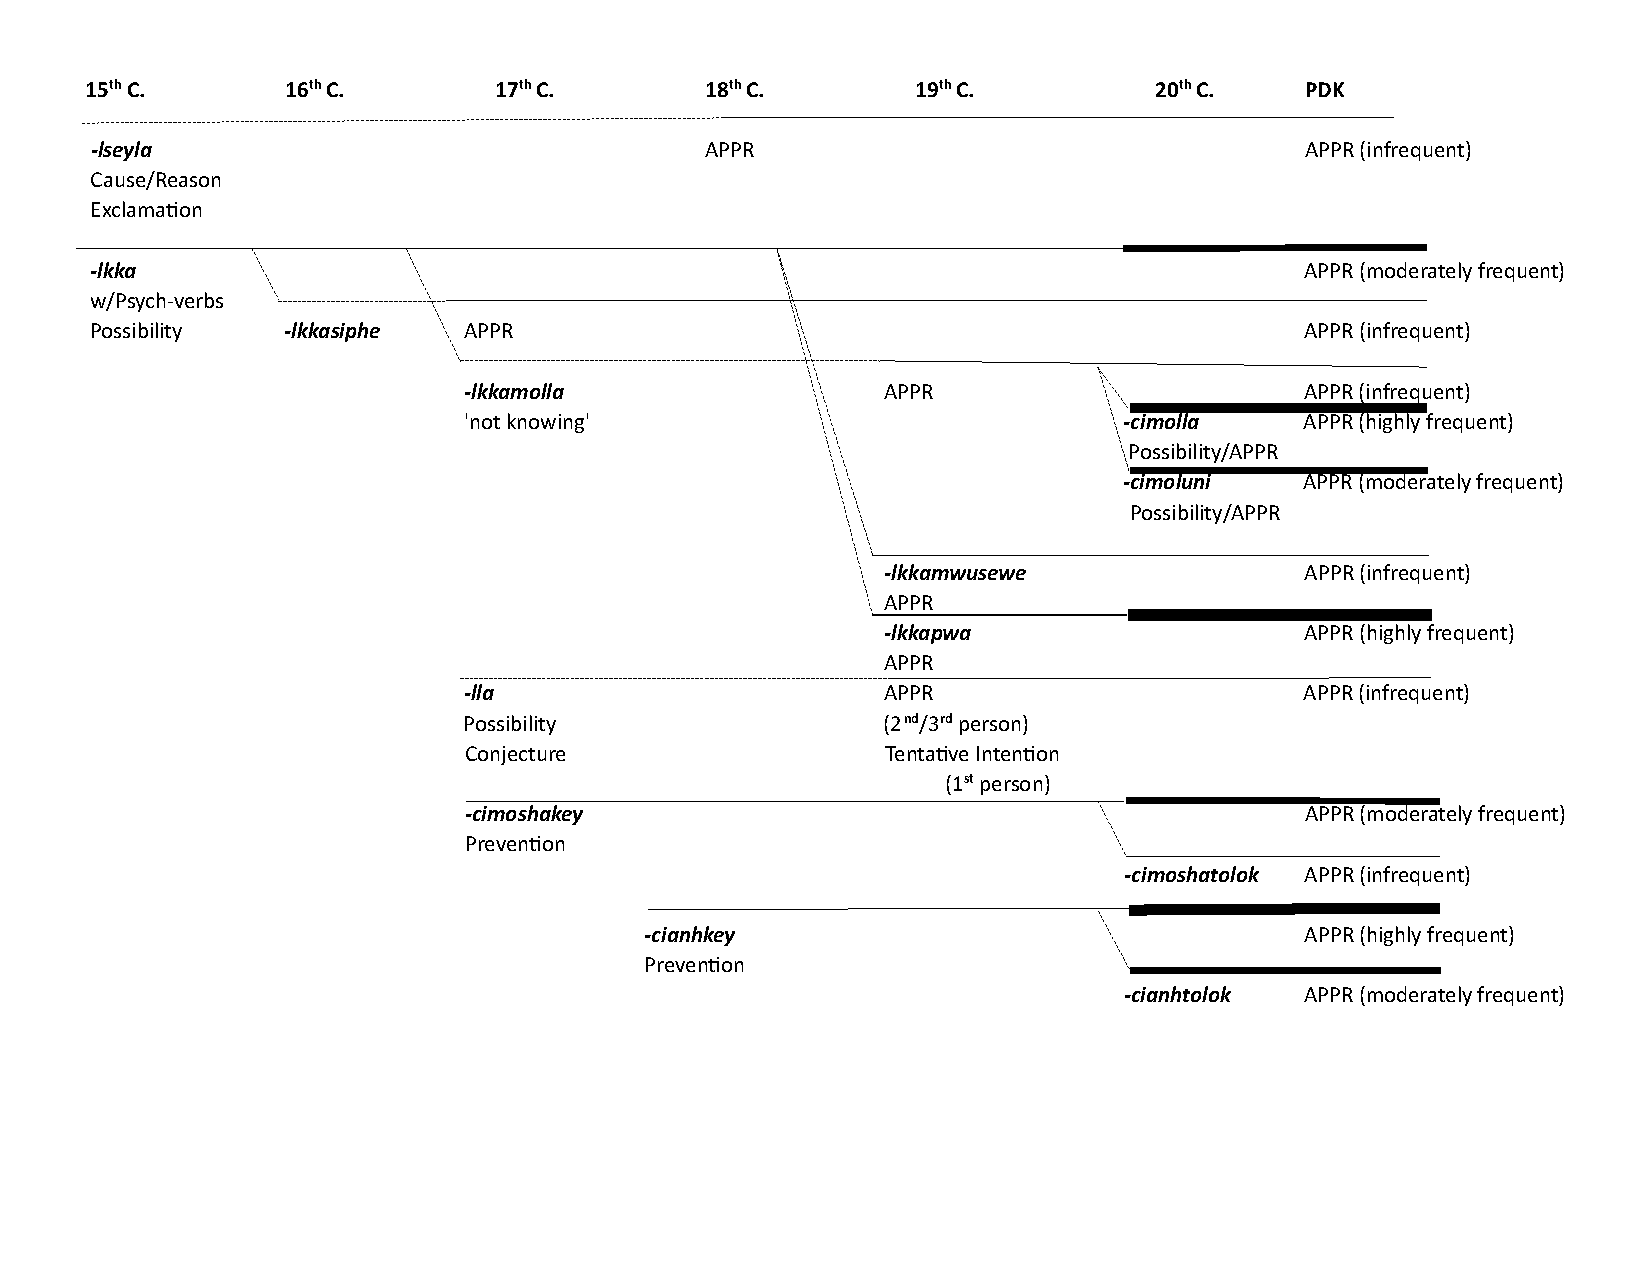
\includegraphics[width=1.0\textwidth]{figures/RK_Fig1_new.pdf}
     %\includegraphics[height=.5\textheight]{figures/figure_treis_1corr.png}
    \caption{Historical development of apprehensionals}
    \label{fig:RK_Fig1_new}
\end{sidewaysfigure}


When multiple forms carry an identical or similar function, there occurs functional tension among them and certain forms may gain functional primacy over others, pushing other competitors outside the functional domain or into other genre- or register-specific usage within the domain. This process has been termed ``specialization" \citep{Hopper1991}. From a statistical analysis of the frequency in the Modern Korean corpus, the primary apprehensional is \nobreakdash-\textit{lkkapwa}, with 276 occurrences per million words. It is followed by \nobreakdash-\textit{cianhkey} (123 pmw) and \nobreakdash-\textit{cimolla} (55 pmw).  The relative functional strengths of the apprehensionals in PDK are graphically presented in \figref{fig:RK_Fig2_new}.


\begin{figure}

    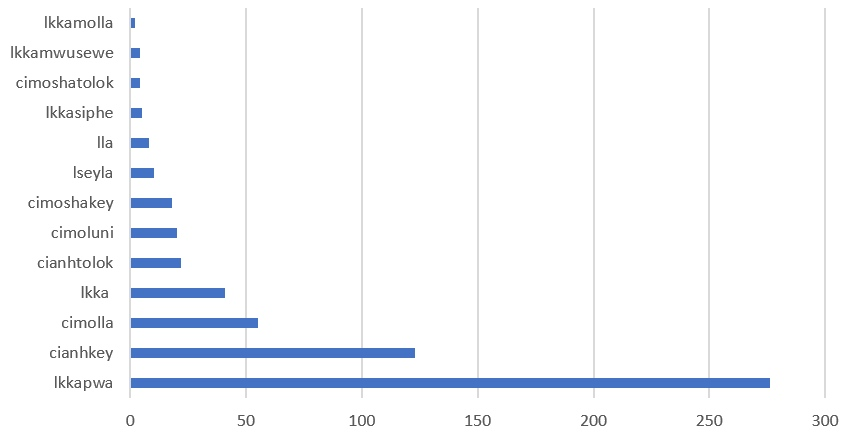
\includegraphics[width=0.96\textwidth]{figures/RK_Fig2_new.jpeg}
    \caption{Frequency of apprehensionals in PDK (Drama-Movies corpus)}
    \label{fig:RK_Fig2_new}
\end{figure}


From \figref{fig:RK_Fig1_new} and \figref{fig:RK_Fig2_new}, one notable aspect of the divergence and specialization patterns is that the most frequent apprehensionals in PDK are not those with the longest history of grammaticalization. Conversely, those with the shortest history are not the least frequent in PDK. For instance, the most frequently used apprehensionals such as \nobreakdash-\textit{lkkapwa}, \nobreakdash-\textit{cianhkey}, and \nobreakdash-\textit{cimolla} came to be used as apprehensionals only from the 19\textsuperscript{th}, 18\textsuperscript{th}, and 20\textsuperscript{th} century onwards, respectively, whereas the least frequently used apprehensionals such as \textit{\nobreakdash-lkkamolla, \nobreakdash-lkkamwusewe,} and \nobreakdash-\textit{cimoshatolok} developed into apprehensionals from the 17\textsuperscript{th}, 19\textsuperscript{th}, and 17\textsuperscript{th} century, respectively.

Also important in this context is the notion of the degree of grammaticalization. Even though instances of grammaticalization are often discussed as of variable degrees, e.g.\  ``highly" grammaticalized, ``weakly" grammaticalized, etc., there is no established method to measure the degree of grammaticalization. We may use the four parameters discussed above, i.e., desemanticization, extension, decategorialization and erosion, to examine how much change has occurred along these parameters. Alternatively, \citegen{Lehmann2015} six parameters may serve as a diagnostic, i.e., the degree of attrition (reduction of semantic content and/or phonetic substance), paradigmaticization (decrease of the paradigm size), obligatorification (use increasingly becoming obligatory), condensation (narrowing of structural scope), coalescence (increase of bondedness), and fixation (reduction of syntagmatic variability). Either way, however, since the parameters operate at different domains of grammar, such as phonology, morphology, semantics, and syntax, and since the source concepts may already be grammaticalized to some degree, different levels of change cannot be quantified for direct comparison in determining relative degrees of grammaticalization across parameters. These practical problems notwithstanding, we can hypothesize, following \citet[106]{HopperTraugott2003}, that ``the more frequently a form occurs in texts, the more grammatical it is assumed to be'' and that textual frequency may represent different degrees of grammaticalization of multiple forms in the same or similar functional paradigm (see, however, \citealt{Heine1992} for discussion of exceptions as well as \citealt[38--39]{HeineKuteva2007} for the lack of a clear correlation between frequency and grammaticalization).

From this perspective, the state of affairs of the Korean apprehensionals suggests that \nobreakdash-\textit{lkkapwa} is the most grammaticalized and \nobreakdash-\textit{lkkamolla} is the least grammaticalized, and further that the historical depth and the degree of grammaticalization are not coextensive.



\subsection{The role of source concepts}
\label{subsec:sourceconcepts}

The role of source semantics in grammaticalization is crucial because grammaticalization is basically a conceptually motivated process (\citealt{Heine1986,Heine1997,HeineClaudi1986,HeineEtAl1991,Kuteva2001}). We noted in \sectref{subsec:appinKorean} that there is a certain limited number of concepts that are involved in the source constructions, i.e.\  lexical verbs of perception and cognition such as `see', `be fearful', `not know', and `think' and the grammatical concepts of futurity, question, mode, and purpose. The relation between the source concepts and the resultant grammatical functions has been noted by grammaticalization researchers (cf.\ the source determination hypothesis by \citet{bybeeetal1994}), and we are going to consider the development of apprehensionals in this light.

The contribution of cognitive verbs such as `fear', `not know', and `(be inclined to) think' and the perception verb `see' to the development of apprehension is obvious, since apprehension is an inherently cognitive/perceptual state of affairs (cf.\ ``apprehensional-epistemic" in \citet{lichtenberk1995}). As we noted in \sectref{subsec:futurequestion}, the oldest predecessor construction of apprehensional \nobreakdash-\textit{lkka} in Late Middle Korean was followed by verbs of cognition, e.g.\  `worry', `doubt', `lament', etc. (see \textsf{§}2.2 for a more extensive list), while \nobreakdash-\textit{lkka} was only a combination of the future marker (-\textit{l}-) and the interrogative sentence-ender (-\textit{kka}). When the internal cohesion in the collocation increased, the collocational constructions became formally univerbated and conceptually integrated into the set of apprehensionals, thus leading to the emergence of multiple apprehensionals, e.g.\  \nobreakdash-\textit{lkkasiphe} (with `think'), \nobreakdash-\textit{lkkamolla} (with `not know'), \nobreakdash-\textit{lkkamwusewe} (with `be fearful of'), and \nobreakdash-\textit{lkkapwa} (with `see').\footnote{Conceptual integration cannot be easily proven with quantifiable criteria. In Korean, however, one such indication appears in the way people write. These apprehensionals are structurally compositional and thus need to be written with inter-lexical spacing according to orthographic rules, but they are often written without spaces at the word boundary in informal writing (e.g., \nobreakdash-\textit{lkkasiphe} instead of \textit{-lkka siphe}; \nobreakdash-\textit{lkkamolla} instead of \textit{-lkka molla}, etc.). Incidentally, disappearance of interlexical spacing is commonly observed in the grammaticalization of multi-word constructions such as auxiliary verbs, complex postpositions, sentence-final particles, etc.}   

It is interesting to note that in the development of apprehensionals from \nobreakdash-\textit{lkka}, the `fear'-semantics of the co-occurring verbs or propositions denoting undesirable events seems to have been absorbed by \nobreakdash-\textit{lkka}, a process whereby \nobreakdash-\textit{lkka} itself became an apprehensional around the 18\textsuperscript{th} century. This is a plausible scenario, a process that \citet{bybeeetal1994} labeled `absorption of contextual meaning' and included among the possible grammaticalization mechanisms (see \citealt[230--236]{bybeeetal1994} for illustration of modal meanings). Similarly, \citet{Rhee2017} shows that the semantics of many sentence-final particles that developed from insubordination are in fact the inferred meanings of the imagined reconstruction of an elided main clause, instances of borrowed semanticization from neighboring forms. A caveat is that the process of borrowed semanticization or absorption has not happened in full, and as a result there are non-apprehensional usages of \nobreakdash-\textit{lkka} in PDK (see \sectref{subsec:futurequestion}). 

Another important aspect of the contribution of source semantics is that not only the lexical semantics but also grammatical concepts associated with the source constructions are important contributors. It is evident that futurity plays an important role in the development of apprehensionals, as shown by the fact that seven out of thirteen developed from constructions containing the future tense marker \nobreakdash-\textit{l}-. The semantics of the particles for mode (-\textit{key}) and purpose (\nobreakdash-\textit{tolok}), each involved in two apprehensionals, is also inherently futuristic, in the sense that the event marked by them is intended by the (implied) sentential subject but has not yet been realized. Interrogative marking also plays an important role.\footnote{The connective \nobreakdash-\textit{key}, also often referred to as a converb marker, is polyfunctional but its primary function is marking the mode of the action or state denoted by the verb \citep{Rhee1996}. For diverse functions of  \nobreakdash-\textit{key} in grammaticalized constructions, see \citet{Kim2011}.} Five of the apprehensional markers have the question marker \nobreakdash-\textit{kka} as a component. The grammatical notions of futurity and interrogative are significant because they bring forth the notions of uncertainty and indeterminateness, which, in turn, engender the notion of apprehension. It is true that the source of apprehension does not have to be uncertainty, considering that we may become particularly apprehensive when we are positive that something bad is going to happen.\footnote{We thank an anonymous reviewer who brought this insightful point to our attention.} However, it is also true that the uncertainty-anxiety relationship has long been recognized in human psychology and neuroscience. For instance, it has been noted that the human brain is an ``anticipation machine'' (\citealt{Gilbert2006}, as cited in \citealt[488]{GrupeNitschke2013}), and that people have a general propensity toward negative affective responses to uncertainty (\citealt{AndersonEtAl2019}, see also \citealt{Carleton2016b, Carleton2016a,}). 


\subsection{Pragmatic inference, reinterpretation, and subjectification}
\label{subsec:pragmatic}

It is widely recognized that grammaticalization often results from pragmatic inference (\citealt{Traugott1989,HopperTraugott2003,Slobin1994,bybeeetal1994,Fischer2008}, and numerous others). The process can be illustrated with the apprehensional connective \nobreakdash-\textit{lkkapwa}, developed from \textit{-l-kka-po-a} [\textsc{fut-q}-see-\textsc{conn}], exemplified in \REF{ex:RK1b}, with modification:


\ea \label{ex:RK17} \textnormal{Connective} \textit{-lkkapwa} \textnormal{`for fear of'} \\
\ea \label{ex:RK17a}
\gll Ku-nun cencayng-i na-lkkapwa cam-ul mos ca-n-ta. \\
he-\textsc{top} war-\textsc{nom} come.out-\textsc{appr} sleep-\textsc{acc} cannot sleep-\textsc{prs-decl} \\
\glt `He cannot sleep for fear of a war.' \\
\ex \label{ex:RK17b}
\gll Ku-nun cencayng-i na-l-kka pw-a cam-ul mos ca-n-ta. \\
he-\textsc{top} war-\textsc{nom} come.out-\textsc{fut-q} see-\textsc{conn} sleep-\textsc{acc} cannot sleep-\textsc{prs-decl} \\
\glt Lit.\ `As he sees/saw (it), (saying,) ``Will a war break out?'', he cannot sleep.'
\z
\z


 Before the poly-morphemic \nobreakdash-\textit{lkkapwa} was fully grammaticalized, the meaning of the example \REF{ex:RK17a}, based on the components constituting \nobreakdash-\textit{lkkapwa}, would have been \REF{ex:RK17b}, `As he sees/saw (it), (saying,) ``Will a war break out?'', he cannot sleep.' This interpretation, faithful to the meanings of the source components, makes reference to `his seeing (or having seen) something'. However, since the war has not (yet) broken out, actual occurrence of visual perception of the war is not likely. Probable events may be only hearing rumors about a war or sensing the possibility in one way or another. Therefore, making reference to seeing (by using the verb \textit{po}- `see') may be interpreted by the hearer as either a hyperbole or a metaphor of expressing a cognitive state (i.e.\  knowledge) by means of bodily perception (i.e.\  seeing), a crosslinguistically common instance of metaphorization (see \citealt{LakoffJohnson80,Sweetser1990}). 

Also, it is not clear if the referent of \textit{ku-nun} `he' in \REF{ex:RK17a} really uttered the question ``Will a war break out?'' In fact, it is not likely that the question was actually asked by him, because \nobreakdash-\textit{lkka} as a regular future interrogative marker (not as an apprehensional) is typically a monologic sentence-ender (a type of ``audience-blind" form, \citealt[105]{RheeKoo2017}).\footnote{For this characteristic of the sentence-ender \nobreakdash-\textit{lkka}, the clause headed by \nobreakdash-\textit{lkkapwa,} embedding a question thus marked, represents a situation in which the sentential subject is asking a monologic question to himself/herself while looking at an event or state.} In other words, the speaker imagines that the sentential subject of an apprehensional sentence asks himself or herself if something will happen. Thus, the question exists only in the mind of the speaker. In this process, the sentence-ender of the question in the future tense is pragmatically reinterpreted as a connective of a clause that marks the cause of apprehension. This type of figurative hyperbole is a common expressive strategy in Korean lexicalization and grammaticalization, observed by \citet{Rhee2009}, who labels it a ``through a borrowed mouth" phenomenon.\footnote{\citet{Rhee2009} lists descriptive adverbials that originated from quotation constructions, e.g., \textit{cwuk-keyss-ta-ko} `saying ``I will die''' to \textit{cwukkeysstako} `desperately', \textit{michyess-ta-ko} `saying ``I am insane''' to \textit{michyesstako} `nonsensically', etc. The quotations ``I will die", ``I am insane" did not originate from the person being described but from the imagination of the observer.} What is noteworthy is that all this expressive enrichment involves pragmatical inference, i.e., from ``a question is a speech act involving the speaker's uncertainty" to ``uncertainty about the future generates fear" and further to ``a question about the future marks fear".

Pragmatic inference may well -- but does not have to -- lead to subjectification, a process whereby ``meanings based in the external described situation [become] meanings based in the internal (evaluative/perceptual/cognitive) situation'', or ``meanings tend to become increasingly situated in the speaker's subjective belief-state/attitude toward the situation'' \citep[208--209]{TraugottKönig1991}, a frequent semantic concomitant in grammaticalization \citep{Traugott2003}. In this light, the semantic/functional change through pragmatic inference described above is a paradigm example of subjectification, i.e., the change from `as one sees something and asks ``Will x occur?''' to `for fear of x' is a shift from a description of the world (i.e., the external described situation) to one of a mental world (i.e., the meaning situated in the speaker's subjective attitude).

Similarly, the development of apprehension from uncertainty and indeterminateness is a clear instance of subjectification. Uncertainty is a cognitive state often resulting from the indeterminateness of a situation, whereas apprehension is more subjective by virtue of being an affective state. Even when apprehensionals do not mark fear but potential undesirability, the evaluative judgment of a future event involves subjectivity.\footnote{It is noteworthy in this context that \citet{Kim2021} notes in her analysis of \nobreakdash-\textit{ltheyntey} from a connective (e.g., `while P will occur') to a final particle (e.g., `It is regrettable that P') that the grammaticalization involves semantic extension into wishing, regretting, worrying, etc., in which conjecture and context play important roles.} Similarly, the development of the verb \textit{molu}- `not know' to the apprehensionals \nobreakdash-\textit{lkkamolla, -cimolla,} and \nobreakdash-\textit{cimoluni} is an instance of subjectification, along the series of changes as `have no knowledge' > `be unsure' > `be uncertain' > `be worrisome' > `be apprehensive'. The series of changes along the conceptual continuum strongly suggests developmental directionality from epistemic possibility to apprehension (\citealt{Dobrushina2006,pakendorfschalley2007}, among others).

When pragmatic inferences occur, often involving subjectification, there also occur morphosyntactic reanalysis and functional reinterpretation, i.e., a poly-morphemic construction with compositional meaning being reanalyzed as a single form with grammatical meaning. Certain types of morphosyntactic change can result in much more drastic consequences. For instance, we noted in \sectref{subsec:appinKorean} that the resultant grammatical category (i.e.\  connective or sentence-ender) of most instances of apprehensionals is identical with the grammatical category of the final element in the source construction and that there are three exceptional cases, i.e.\  \nobreakdash-\textit{lkka, -lla}, and \nobreakdash-\textit{lseyla} ((a), (f), and (g) in \tabref{tab:apprehensionalforms}). They all end with a sentence-ender: \nobreakdash-\textit{lkka} with an interrogative sentence-ender \nobreakdash-\textit{kka}, and \nobreakdash-\textit{lla} and \nobreakdash-\textit{lseyla} with a declarative sentence-ender with some nuance of exclamative, \nobreakdash-\textit{la}. However, \nobreakdash-\textit{lkka} is now an apprehensional connective, not an apprehensional sentence-ender, and \nobreakdash-\textit{lla} and \nobreakdash-\textit{lseyla} end with a sentence-ender \nobreakdash-\textit{la} but now as apprehensionals they also function as connectives. This state of affairs warrants some discussion.

The source construction of \nobreakdash-\textit{lkka}, as noted in \sectref{subsec:futurequestion}, is an interrogative sentence in the form of direct quotation, i.e.\  an embedded question. However, when the direct quote provides a cause/reason as the background of the main clause, the form at the boundary of embedding, i.e.\  the end of the embedded sentence, \nobreakdash-\textit{lkka}, is functionally reinterpreted as a causal connective (linking the state or event feared by the speaker or the sentential subject to its consequence). Let us look at the following example \REF{ex:RK18}:


\ea \label{ex:RK18}
\ea \label{ex:RK18a}
\gll Cencaying-i na-l-kka cam-i an o-n-ta. \\
war-\textsc{nom} come.out-\textsc{fut-q.end} sleep-\textsc{nom} not come-\textsc{prs-decl} \\
\glt `Will a war break out? (I) cannot go to sleep.' \\
\ex \label{ex:RK18b}
\gll Cencaying-i na-lkka cam-i an o-n-ta. \\
war-\textsc{nom} come.out-\textsc{appr.conn} sleep-\textsc{nom} not come-\textsc{prs-decl} \\
\glt `(I) cannot sleep for fear of a war (breaking out).'
\z
\z

\noindent The change from \REF{ex:RK18a} to \REF{ex:RK18b} clearly shows the inter-clausal morphosyntactic reanalysis of regarding the sentence-final \textit{-l-kka} as a clause-final connective and functional reinterpretation of regarding the marker of a question with respect to the future as a marker of apprehension, thus from a sentence-ender to a connective. As a matter of fact, this type of change is pervasive in the grammaticalization of connectives in Korean, which involves ``self-quotative constructions" (SQCs) \citep[256]{KooRhee2019}, \nobreakdash-\textit{lkka} being one of them. Example \REF{ex:RK19} illustrates the SQC connective \nobreakdash-\textit{na}, whose original function is marking an interrogative sentence, just like the apprehensional \nobreakdash-\textit{lkka} being discussed here:

\ea \label{ex:RK19}
\ea \label{ex:RK19a} \textnormal{Connective (causal)} \textit{-na} \\
\gll Amwu-to eps-\textbf{na} coyongha-ta. \\
anyone-even not.exist-\textsc{\textbf{conn}} be.quiet-\textsc{decl} \\
\glt `It's quiet, perhaps because there's nobody around.' \\
\ex \label{ex:RK19b} \textnormal{Source construction \textit{-na} \textsc{`-q'}} \\
\gll Amwu-to eps-\textbf{na} coyongha-ta. \\
anyone-even not.exist-\textsc{\textbf{q}} be.quiet-\textsc{decl} \\
\glt Lit.\ {`}``Is nobody here?'' it is quiet.' \citep[267]{KooRhee2019} \\
\z
\z


\noindent The source-construction example \REF{ex:RK19b} consists of two sentences: one monologic question and one (subject-less) declarative sentence. It is noteworthy that two juxtaposed sentences of this type can undergo coalescence \citep{Haspelmath2011} into a single sentence (as in \REF{ex:RK19a}). In this process, the sentence-final element (the question particle \nobreakdash-\textit{na} in \REF{ex:RK19b}) develops into a connective (the causality marker in \REF{ex:RK19a}). The examples in \REF{ex:RK19} show a change analogous to the one with \nobreakdash-\textit{lkka}, from a sentence-ender to a connective; specifically, from a question marker to a causal connective (note, however, that \nobreakdash-\textit{na} does not encode apprehension).

A similar pattern is also observed in the development of apprehensional connectives from apprehensional sentence-enders, such as \nobreakdash-\textit{lla} and \nobreakdash-\textit{lseyla}.  The apprehensionals \nobreakdash-\textit{lla} and \nobreakdash-\textit{lseyla} end with a sentence-ender \nobreakdash-\textit{la} in their source constructions. Previous studies analyze them as sentence-enders (\citealt{Ramstedt1997,Kim1960,Ko2002,Jang2002}). Let us look at the example \REF{ex:RK10} illustrating the apprehensional \nobreakdash-\textit{lla}, repeated here for convenience as \REF{ex:RK20a}:



\ea \label{ex:RK20}
\ea \label{ex:RK20a} \textnormal{$[$In preparation of a funeral$]$} \\
\gll Pang tewu-lla pwul st\textsc{a}y-cimal-ko ko-y tuleka-lla kwistol mak-el\textsc{a}. \\
room be.hot-\textsc{appr} fire make-\textsc{proh}-and cat-\textsc{nom} enter-\textsc{appr} flue.opening block-\textsc{imp} \\
\glt `Don't make fire (for floor-heating) lest the room become too hot (for the corpse), and block the flue opening lest a cat enter (through it) [which is ominous according to superstitions].' (ca.\ 1870 \textit{Pakhungpoka})
\ex \label{ex:RK20b}
\gll Pang tewu-\textbf{l-la} pwul st\textsc{a}y-cimal-ko ko-y tuleka-\textbf{l-la} kwistol mak-el\textsc{a}. \\
room be.hot-\textsc{\textbf{fut-end}} fire make-\textsc{proh}-and cat-\textsc{nom} enter-\textsc{\textbf{fut-end}} flue.opening block-\textsc{imp} \\
\glt `I'm afraid the room will become too hot. Don't make fire (for floor-heating), and I'm afraid a cat will enter. Block the flue opening.'
\z
\z


\noindent The translation \REF{ex:RK20a} of the example is based on the interpretation of \nobreakdash-\textit{lla} as a connective. If we follow the analyses referenced above, the example would be translated as \REF{ex:RK20b} with the structure of: [\textsubscript{S1} I'm afraid the room will become too hot.] [\textsubscript{S2} Don't make fire (for floor-heating)], and [\textsubscript{S3} I'm afraid a cat will enter.] [\textsubscript{S4} Block the flue opening.], containing four finite sentences, with S2 and S3 constituting a coordinated sentence, combined by the coordinating connective \nobreakdash-\textit{ko} `and'. Note, however, that conceptual cohesion does not exist between S2 and S3. Instead, the conceptual cohesion is found between S1 and S2, and between S3 and S4, respectively. In other words, S1 is the reason for saying S2, and S3 for saying S4. The connections between S1 and S2 and between S3 and S4 are pragmatic causality or ``enablement" (cf.\ \citealt[77]{Sweetser1990}).\footnote{In her discussion of conjunctions with an example of ``What are you doing tonight, because there's a good movie on,'' \citet[77]{Sweetser1990} interprets the function of the causal conjunction \textit{because} as a means of justifying and enabling the question, thus the cause of speech act.} Therefore, the example is better analyzed as a sentence constituting two sentences in coordination, each consisting of a subordinate clause and an imperative main  clause: [\textsubscript{S}[\textsubscript{S1}[\textsubscript{SUB.CL} Reason-\textsc{appr.conn}] [\textsubscript{MAIN.CL} Command]]-\textsc{coord} [\textsubscript{S2}[\textsubscript{SUB.CL} Reason-\textsc{appr.conn}] [\textsubscript{MAIN.CL} Command]]]. In other words, the connective interpretation in \REF{ex:RK20a} is better than the sentence-ender interpretation in \REF{ex:RK20b}. This situation is closely related to the crosslinguistic observation that apprehensionals are often used in the contexts of ``imperative indicating the action the hearer should undertake to avoid the unpleasant outcome'' and ``prohibitive indicating the action the hearer should avoid'' \citep{Schultze-Berndt2015} and that apprehensionals are linked to warning/threat and negative command (prohibitive) (\citealt{pakendorfschalley2007}, as cited in \citealt{Schultze-Berndt2015}).

Therefore, the pragmatic motivation for attributing a causal relation between two sentences and for redefining the grammatical status of the sentences seems to have led to the reanalysis of a former sentence-ender into a connective. This type of reanalysis has occurred in the grammaticalization of former sentence-enders into connectives (as shown in \REF{ex:RK19} and \REF{ex:RK20} above, and conversely, and more frequently, in the grammaticalization of former connectives into sentence-enders through the processes of \textit{insubordination} (\citealt{evans2007,EvansWatanabe2016}) and \textit{incoordination} \citep{KutevaEtAl2015,KutevaEtAl2017}. In fact, pragmatic inferences that operate in insubordination and incoordination prompted the functional extension of some apprehensional connectives to the paradigm of sentence-final particles, marking tentative intention, doubt, indeterminateness, possibility, etc.  \citep{KooRhee2001,KooRhee2013,Sohn2003,RheeKoo2017}.



\section{Summary and conclusion}
\label{sec:rhee:summary}

Despite the fact that Korean has a large number of apprehensionals, their developmental paths have not received any serious analysis to date. As we intended to address all apprehensionals being used in PDK, we were unable to trace all the grammaticalization trajectories of the individual forms diachronically, but we have shown that Korean apprehensionals have differential historical depths and varying degrees of specialization. They form multiple layers in the functional domain of apprehensionals in PDK.

Among the four main interrelated grammaticalization mechanisms (\citealt[2]{HeineKuteva2002}), i.e., desemanticization, extension, decategorialization, and erosion, erosion is the least prominent one. Unlike highly grammaticalized markers which tend to be short in form, many apprehensionals are still at the periphrastic stage in morpho-syntactic terms. This suggests that apprehensional markers in Korean have not acquired the status of full-fledged apprehensionals. In fact, many of them can still be used for non-apprehensional functions. This functional split is prominent in their use as an apprehensional connective and as a non-apprehensional sentence-ender. Further, some apprehensionals originated from structurally complex constructions through strengthening of pragmatic inferences based on the semantics of the components, notably epistemic modals, whereas the `fear'-based apprehensionals incorporated a `fear' verb and thus their apprehensional function was visible throughout their history. Multiple forms synchronically layered in the functional domain of apprehensionals have variable specializations as shown in their frequency of use. 

Lexical semantics as well as the functions of grammatical forms in the source constructions contributed to the creation of the notion of apprehension. Of particular importance are (i) the perception/cognition verbs denoting `be fearful', `not know', `think', and `see' in the lexical sources, and (ii) futurity, interrogative, mode and purpose from the grammatical formants.

In the course of development of apprehensionals, pragmatic inferences, subjectification, morphosyntactic reanalysis, and functional reinterpretation are prominent driving forces. In particular, the cross-categorial flexibility between connectives and sentence-enders is largely due to the pragmatic motivations that attribute a causal relation between two sentences and redefine the grammatical status of the sentences. These developmental patterns are not isolated instances but are commonly attested in the grammaticalization scenarios involving insubordination and incoordination in the history of Korean. 


\section*{Abbreviations}
\begin{tabularx}{.5\textwidth}{@{}lQ@{}}
\textsc{acc} & accusative \\
\textsc{adn} & adnominalizer \\
\textsc{appr} & apprehensional \\
\textsc{ben} & benefactive \\
\textsc{comp} & complementizer \\
\textsc{conj} & conjecture \\
\textsc{conn} & connective \\
\textsc{decl} & declarative \\
\textsc{end} & sentence-ender \\
\textsc{fut} & future \\
\textsc{gen} & genitive \\
\textsc{hon} & honorific \\
\textsc{imp} & imperative \\
\textsc{ind} & indicative \\
\textsc{mode} & mode-adverbializer\end{tabularx}%
\begin{tabularx}{.5\textwidth}{@{}lQ@{}}
\textsc{nom} & nominative \\
\textsc{nomz} & nominalizer \\
\textsc{opt} & optative \\
PDK & present day Korean \\
\textsc{pl} & plural \\
\textsc{prog} & progressive \\
\textsc{proh} & prohibitive \\
\textsc{prs} & present\\
\textsc{pst} & past \\
\textsc{purp} & purposive \\
\textsc{q} & question particle/marker \\
\textsc{retro} & retrospective \\
\textsc{top} & topic \\
\textsc{voc} & vocative \\\\
\end{tabularx}

\section*{Acknowledgements}
We are thankful to the anonymous reviewers of the manuscript and to Eva Schultze-Berndt, Marine Vuillermet, and Martina Faller for their constructive comments and suggestions. This work was supported by the Ministry of Education of the Republic of Korea and the National Research Foundation of Korea (NRF-2020S1A5A2A03043203).




\printbibliography[heading=subbibliography,notkeyword=this]
\end{document}
